\documentclass[bibliography=totocnumbered]{scrartcl}
\usepackage{imakeidx}
\usepackage{ragged2e}
\usepackage{setspace} % Um den Zeilenabstand zu ändern.
\usepackage{gensymb}
%\usepackage{authblk}
% \usepackage{minitoc} % for the chpaters
\usepackage{wasysym}
%\usepackage{SI}
\usepackage{array} % Verwendung von Matrizen
\usepackage{booktabs} % Schöne Tabellen beziehungsweise sie sehen damit professioneller aus.
\usepackage{tabulary} % Ähnlich wie tabularx, ermöglicht aber das ändern der Ausrichtung der Spalten.
\usepackage{tabularx} % Tabellen mit automatischen Zeilenumbruch.
\usepackage{enumitem}
\usepackage{physics}
\usepackage[T1]{fontenc}% fontec und inputenc ermöglichen
\usepackage{graphicx}%Für Grafiken
\usepackage{rotating} % lässt Grafiken rotieren
\usepackage{mathtools}% mathematische Werkzeuge
\usepackage{amsmath}% Mathetools
\usepackage{amsfonts}% Mathetools
\usepackage{amssymb}% Symbole wie Natürliche Zahlen
\usepackage{geometry}
%\usepackage{bibtex} 
\usepackage{tablefootnote}% Fußnoten in Tabellen
\usepackage{float}% für eingebundene Bilder
\usepackage{fancyhdr} % Seiten schöner gestalten, insbesondere Kopf- und Fußzeile
\usepackage{ulem} 
\usepackage{dcolumn}% Align table columns on decimal point
\usepackage{bm}% bold math
\usepackage[ngerman]{babel} % Worttrennung nach der neuen Rechtschreibung und deutsche Bezeichnungen. babelfunktion wird wegen Literatur gebraucht.
\usepackage{subfloat} % Was macht diese Packet?
\usepackage{caption} % Unter-/Überschriften für Bilder, Grafiken und Tabellen
\usepackage{subcaption}
\usepackage{txfonts}
\usepackage{titling}% Titel
\usepackage[style=alphabetic]{biblatex} %biblatex mit alphabetic laden. alphbetic=Zitationsstil
\usepackage{bookmark}
\usepackage[printonlyused]{acronym}
\usepackage{amsthm}
\usepackage{pdfpages}
\usepackage{tikz}
\usepackage[siunitx,americanvoltages, europeanresistors,americancurrents]{circuitikz}
\usepackage{listings}
\usepackage{abstract}
\usepackage[per-mode = fraction]{siunitx}
\usepackage{hyperref}
\newcommand{\R}{\mathbb{R}} % reelle Zahlen
\newcommand{\N}{\mathbb{N}} % natürliche Zahlen
\newcommand{\C}{\mathbb{C}} % komplexe Zahlen
\newcommand{\Q}{\mathbb{Q}} % rationale Zahlen
\newcommand{\Z}{\mathbb{Z}} % ganze Zahlen
\newcommand{\F}{\mathbf{F}} % Kraft
\newcommand{\E}{\mathbf{E}} % Energie
\newcommand{\V}{\mathbf{v}} % Geschwindigkeit
\newcommand{\B}{\mathbf{B}} % magnetischer Fluss
\newcommand{\J}{\mathbf{j}} % Stromdichte ?
\newcommand{\D}{\mathbf{D}} % elektrische Induktion
\newcommand{\HH}{\mathbf{H}} % magnetische Feldstärke
\newcommand{\M}{\mathbf{M}} % Magnetisierung
\newcommand{\p}{\mathbf{P}}
\newcommand{\rr}{\mathbf{r}}
\newcommand{\vp}{\varphi}
\newcommand{\ve}{\varepsilon}
\newcommand{\vcc}[1]{\left(\begin{matrix}#1\end{matrix}  \right)}
\newcommand{\m}[1]{\left\lbrace #1\right\rbrace}
\newcommand{\los}{\noindent\textbf{Lösung}:}
\newcommand{\rang}[2]{\text{Rang}(#1)=#2}
\newcommand{\vpe}{\frac{1}{4\pi\ve_0}}
\newcommand{\qvpe}{\frac{q}{4\pi\ve_0}}
\newcommand{\geg}{\ac{geg.}}
\newcommand{\ges}{\ac{ges.}}

\newcommand{\kommando}[1]{$\backslash$\textit{#1}}
\newcommand{\com}[1]{$\backslash$\textit{#1}$\left\lbrace\ldots\right\rbrace$}
\newcommand{\Com}[2]{$\backslash$\textit{#1}$\left\lbrace #2\right\rbrace$}
\newcommand{\NeuKommando}[2]{$\backslash \textit{#1} \left\lbrace \backslash \textit{#2}\right\rbrace$}
\newcommand{\latex}{\LaTeX $\;$}


% si unitx
\DeclareSIUnit\litre{l}

\hypersetup{
	colorlinks=true,
	linkcolor=blue,
	filecolor=magenta,      
	urlcolor=cyan,
	citecolor=lime!50!black,
	filecolor=red
}
%\addbibresource{} %Bibliographiedateien laden
\addbibresource{bib.bib}

\geometry{a4paper, left=25mm, right=25mm, top=30mm, bottom=30mm}
\lhead{\thedate}
\rhead{GPR}
\lhead{\thetitle}
\pagestyle{fancy}

\usetikzlibrary{patterns}
\usetikzlibrary{3d}
\makeindex[title=Stichwortverzeichnis,intoc
,options= -s Index-Formatierung.ist
]
\author{Ben J. F.}
\allowdisplaybreaks

\lstset
{ %Formatting for code in appendix
    basicstyle=\footnotesize,
    numbers=left,
    stepnumber=1,
    showstringspaces=false,
    tabsize=2,
    breaklines=true,
    breakatwhitespace=false,
}


\title{F4 \\ Bestimmung von Federkonstanten}
\date{27.05.2021}

\begin{document}
	\newgeometry{left=14mm, right=13.5mm, top=60mm, bottom=30mm}
	\begin{titlepage}
		\begin{center}
			{\huge{Grundpraktikum}}\\\vspace*{15mm}
			{\huge{\textbf{\thetitle}}}\\\vspace*{20mm}
			{\theauthor}\\\vspace*{10mm}
			{\thedate}\\\vspace*{40mm}
			
			
			
		\end{center}
	\end{titlepage}
	\makeatother
	\restoregeometry
	\newpage
	
	\tableofcontents
	\newpage
	
	\listoffigures 
	\listoftables
	\newpage
	
	
	
	\section{Motivation und theoretische Vorbetrachtung}
	Ziel dieses Experimentes ist es, die Federkonstante k zu bestimmen, die aus der Federkraft entsteht aufgrund der Auslenkung x.
	\begin{equation}\label{eq: Federkraftglg}
		F_{F}=kx
	\end{equation}
	Dabei unterscheiden wir zwischen der dynamischen und statischen Messung. Die statistische Messung bedeutet, dass die Feder in Ruhe ist und zum Bespiel im Schwerefeld der Erde ist.
	\begin{equation}\label{eq: statisch Messung}
		x=\dfrac{mg}{k}
	\end{equation}
	Bei der dynamischen Messung siehen wir die Feder als einen harmonischen Oszillator an und dabei entsteht der Zusammenhang:
	\begin{equation}\label{eq: dynamische Messung}
		k=4\pi^{2} \dfrac{m}{T^{2}}
	\end{equation}
	Herleitungen und die weitere theoretische Zusammenhänge sind im Versuchsskript\smartcite{Muller.b} zu lesen.
	
	\section{Aufbau und Versuchsbeschreibung}
	\begin{figure}[H]
	    \centering									
		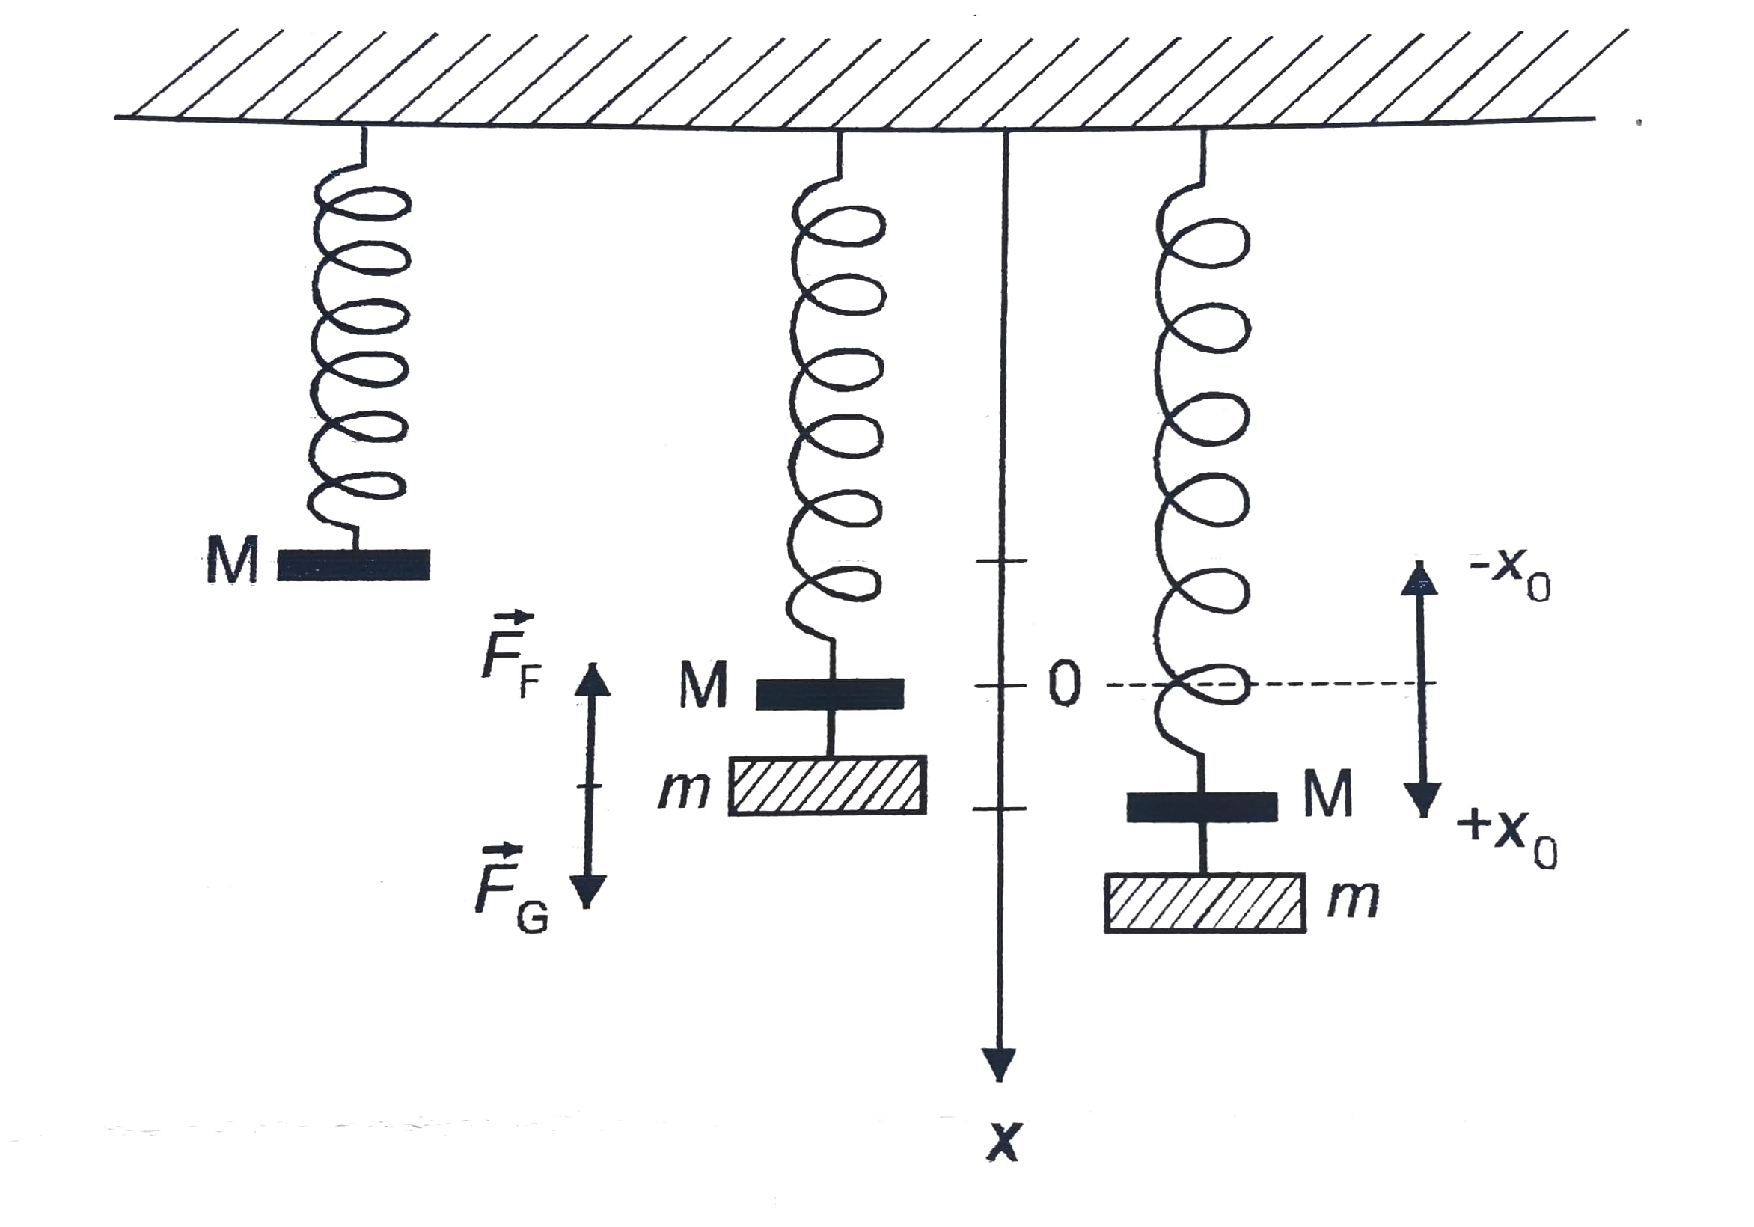
\includegraphics[width=200pt]{fotos/gpr1/VAufbau.pdf}			
		\caption{Aufbau des Versuches zur Bestimmung von Federkonstanten}						
		\label{Abb: Versuchsaufbau}	
	\end{figure}
	
	In dem Experiment wird eine Feder (Masse mf, Torsionsmodul G, Drahtlänge l,
	Drahtdurchmesser d und Wickelradius r) senkrecht zum Boden im Schwerefeld der Erde
	gebracht.
	Im ersten Teilversuch bringen wir 8 Massen $ m $ von ca. 50g nacheinander an die Feder an
	und messen die Auslenkung x, um die statische Messung durchzuführen. Anschließend
	entfernen wir die Massen nacheinander und messen erneut.
	Als nächstes Experiment lassen wir die Feder mit der Masse $ m $ n mal schwingen und
	messen dann die Periodendauer T.
	Als letztes ermitteln wir die Federkonstante k aus den Materialkonstanten:
	\begin{equation}\label{eq: Materialkonstanten}
		k=\dfrac{\pi}{32}\dfrac{G d^{4}}{l r^{2}}
	\end{equation}
	Genauere Angaben und Erklärungen zu dem Aufbau und Versuchsdurchführung ist im
	Versuchsskript\smartcite{Muller.b} zu finden. Die Skizze zum Versuchsaufbau ist in der Abb. (\ref{Abb: Versuchsaufbau}) zu sehen.
	
	\newpage
	\section{Statische Messung}
	In diesem Versuch hängen wir die Massen aus Tabelle (\ref{tab: Massestücke}) an die Feder und bestimmen so die Auslenkung, wie im Aufbau beschrieben.
	\begin{table}[ht!]
		\centering
		\caption{Gewichte der Massestücke von Messplatz 1 und 3}
		\begin{tabular}{|c|c|c|}
			\hline
		Nummerierung	& Messplatz 1 & Messplatz 3 \\
			\hline
			$ m_{1} $& $ (49.818\pm 0.0005) $g & $ (49.995  \pm0.0005) $ g\\
			\hline
			$ m_{2} $& $ (50.342\pm0.0005) $ g& $ ( 50.261 \pm0.0005) $ g\\
			\hline
			$ m_{3} $& $ (50.041\pm0.0005) $g & $ (50.656  \pm0.0005) $ g\\
			\hline
			$ m_{4} $& $ (50.005\pm0.0005) $ g& $ (50.418  \pm0.0005) $ g\\
			\hline
			$ m_{5} $& $(50.723\pm0.0005)  $g & $ (49.930  \pm0.0005) $ g\\
			\hline
			$ m_{6} $& $ (50.516\pm0.0005) $ g& $ (49.970  \pm0.0005) $ g\\
			\hline
			$ m_{7} $& $ (50.609\pm0.0005) $ g& $ ( 50.210 \pm0.0005) $ g\\
			\hline
			$ m_{8} $& $ (50.618\pm0.0005) $ g& $ ( 50.824 \pm0.0005) $ g\\
			\hline
		\end{tabular}
	\label{tab: Massestücke}
	\end{table} 
	\subsection{Datenauswertung}
	Im Material wurde die Masse der Feder mit 5g angegeben und wir addieren diese auf die Messungen. Wir hängen die Massestücke in der Reihenfolge 1 bis 8 an die Feder nacheinander an und hängen diese in umgekehrter Richtung wieder ab.\\
	Dabei ergeben sich folgende Auslenkungen:
	
	\begin{table}[ht!]
		\centering
		\caption{Messwerte statische Messung, \\
			auf die linken Massen wurde die Federmasse hinzugefügt, \\
		bei den rechten Massen nicht}
		\begin{tabular}{|c|c|c||c|c|c|}
			\hline
			Masse [g]& x [cm] auf &x [cm] ab & Masse [g] &x [cm] auf&   x [cm] ab   \\
			\hline
		--	&--  & -- & $ (0\pm 0) $  &0&0 \\
			\hline
			$ 54.818\pm 0.005$&$ 1.00 $  & $ 1.00 $ & $49.995\pm 0.005  $ &$ 1.15$& $  1.05   $  \\
			\hline
			$ 104.16\pm 0.007  $& $ 2.20 $ & $ 2.20  $ & $ 100.256\pm0.007 $ &$ 2.30  $&  $ 2.15  $\\
			\hline
			$ 164.201\pm0.009 $&$ 3.40   $  & $ 3.40   $& $ 150.912\pm0.009 $ &$ 3.25  $&$ 3.15  $   \\
			\hline
			$ 204.206\pm 0.010$&$ 4.60 $  & $ 4.50  $ & $ 201.330\pm 0.010 $ &$ 4.35 $& $ 4.30  $ \\
			\hline
			$ 254.929\pm0.011 $& $ 5.80  $ & $ 5.50  $ & $251.260 \pm0.011 $ &$  5.40  $&$ 5.35  $  \\
			\hline
			$ 305.445\pm 0.012$& $ 7.00  $ & $ 6.60  $ & $301.230 \pm 0.012 $ &$ 6.50  $ & $6.45  $\\
			\hline
			$ 356.054\pm 0.013$& $ 8.10  $ &$ 7.90  $  & $ 351.440\pm 0.013 $ & $ 7.60  $&$ 7.50  $ \\
			\hline
			$ 406.672\pm0.014 $& $ 9.20   $& $ 9.00  $ & $402.264 \pm0.014 $ &$  8.55 $ & $ 8.65  $\\
			\hline
		\end{tabular}
		\label{tab: Mw statische Messung}
	\end{table}
	Aufgrund der Spiegelskala hat man eine Unsicherheit gegeben von
	\begin{equation}
		u_{x}=0.2\text{ mm} + 5\cdot 10^{-4}x \approx 0.05\text{ cm}
	\end{equation}

	Da wir für die ersten beiden x-Spalten von $ (20.00\pm 0.05) $cm abwärts die Skala abgelesen haben und dann die Differenz dazu berechnen, welche in der Tabelle (\ref{tab: Mw statische Messung}) stehen, haben wir für die x-Fehler den folgenden Wert nach Fehlerfortpflanzung:
	\begin{equation}
		u_{x,gesamt}=u_{x}\sqrt{2}=0.07\text{ cm}
	\end{equation}
	Für die letzten beiden x-Spalten haben wir denselben Fehler, mit dem Unterschied, dass wir die Differenz zuerst von $ (19.65\pm 0.05) $cm und dann die Differenz von $ 19.80\pm 0.05 $cm nehmen.\\
	Aus den ersten beiden x-Spalten errechnen wir den Durchschnitt und erzeugen mittels lineare Regression den Graph (\ref{Abb: Reg Sara A1}), wie im Skript\smartcite{MullerPG.2007b}
	erläutert ist. \\
	Aus der Gleichung (\ref{eq: Federkraftglg}) ergibt sich für die lineare Regression:
	\begin{equation}\label{eq: lineare Regression A1}
		x=\dfrac{g}{k}\cdot m+b=a\cdot m+b
	\end{equation}
	Für die dritte x-Spalte ergibt sich der Graph (\ref{Abb: Reg Ben A1 M1}) mit linearer Regresssion und für die vierte x-Spalte ergibt sich der Graph (\ref{Abb: Reg Ben A1 M2}).\\
	Als erstes sollen wir mittels des Steigungsdreiecks des ersten und letzten Wertes die Federkonstante $ k $ bestimmen mit:
	\begin{align}\label{eq: Steigungsdreieck A1}
		k=g \cdot \dfrac{m_{2}-m_{1}}{x_{2}-x_{1}}\\
		u_{k}=k\sqrt{\left(\dfrac{u_{g}}{g}\right)^{2}+\left(\dfrac{u_{m}}{m_{2}-m_{1}}\right)^{2}+\left(\dfrac{u_{x}}{x_{2}-x_{1}}\right)^{2}}
	\end{align}
	Damit ergeben sich für die drei Graphen (\ref{Abb: Reg Ben A1 M1}, \ref{Abb: Reg Ben A1 M2}, \ref{Abb: Reg Sara A1}) folgende Werte:
	
	\begin{table}[ht!]
		\centering
		\caption{k-Werte aus Steigungsdreieck, statische Messung}
		\begin{tabular}{|c|c|c|c|}
			\hline
			& Graph (\ref{Abb: Reg Ben A1 M1}) & Graph (\ref{Abb: Reg Ben A1 M2}) & Graph (\ref{Abb: Reg Sara A1}) \\
			\hline
			Federkonstante $ k $ & $ 46.2\pm 0.5 $ & $ 45.6\pm 0.5 $ & $ 42.1\pm 0.5  $ \\
			\hline
		\end{tabular}
		\label{tab: Fk, Steigungsdreieck, A1}
	\end{table}

\begin{table}[ht!]
	\centering
	\caption{numerische Steigung, statische Messung}
	\begin{tabular}{|c|c|c|c|}
		\hline
		& Graph (\ref{Abb: Reg Ben A1 M1}) & Graph (\ref{Abb: Reg Ben A1 M2}) & Graph (\ref{Abb: Reg Sara A1}) \\
		\hline
		Steigung $ a $ $[\text{cm } \text{kg}^{-1}]  $ & $ 21.26\pm0.15 $ & $ 21.47\pm0.09$ & $ 23.11\pm 0.2 $ \\
		\hline
	\end{tabular}
	\label{tab: Fk, numerisch, A1}
\end{table}
	Die Graphen (\ref{Abb: Reg Ben A1 M1}, \ref{Abb: Reg Ben A1 M2}, \ref{Abb: Reg Sara A1}) bestätigen den linearen Zusammenhang zwischen der Auslenkung und der
	Masse.
	\newpage
	\subsection{Bestimmung der Federkonstanten \\aus den numerischen Anstiegen}
	Es gilt für die Federkonstante gefolgert aus (\ref{eq: Materialkonstanten}) und den gegeben Werten von $ g $ aus dem Versuchsskript\smartcite{Muller.b}.

	\begin{equation}
		k=\dfrac{g}{a}
	\end{equation}
	Und mit der Gaußschen Fehlerfortpflanzung:
	\begin{equation}
		u_{k}=k\sqrt{\left(\dfrac{u_{g}}{g}\right)^{2}+\left(\dfrac{u_{a}}{a}\right)^{2}}
	\end{equation}
	
	\begin{table}[ht!]
		\centering
		\caption{Ergebnisse der Federkonstante $ k $ \\aus dem numerischen Anstieg}
		\begin{tabular}{|c|c|c|c|}
			\hline
			&  Graph (\ref{Abb: Reg Ben A1 M1}) & Graph (\ref{Abb: Reg Ben A1 M2}) & Graph (\ref{Abb: Reg Sara A1}) \\
			\hline
			Federkonstante $ k $ $ [\text{kg s}^{-1}] $& $ 46.2\pm0.3 $ & $ 45.70\pm0.18 $ & $ 42.4\pm 0.4  $\\
			\hline
		\end{tabular}
		\label{tab: k numerisch A1}
	\end{table}
	
	\section{Dynamische Messung}
	Im zweiten Versuchsteil wurde nun die Feder mit der Masse 0.406672 kg zur Schwingung gebracht und die Zeit von 20 Schwingungen 10 mal aufgenommen.
	\subsection{Dynamische Messung für eine Masse}
	
	\subsubsection{Datenauswertung}
	Als Messwerte und grafische Darstellung mittels linearer Regression, der Form y =xa+b, ergibt sich, gemäß Skript\smartcite{MullerPG.2007b}:
	
	\begin{table}[ht!]
		\centering
		\caption{Messwerte Dynamisch für eine Masse}
		\begin{tabular}{|c|c|c|c|c|c|c|c|c|c|c|}
			\hline
			Periodendauer $ T_{20} $ [s] & 11.78 & 11.87 & 11.72 & 11.85 & 11.75 & 12.00 & 11.85 & 11.91 & 11.75 & 11.85 \\
			\hline
		\end{tabular}
		\label{tab: dynamisch für eine Masse}
	\end{table}
	
	Aus diesen wird nun der Durchschnitt bestimmt und mittels lineare Regression der Art
	y = a(x+b) ein Graph erzeugt.
	Aus (\ref{eq: dynamische Messung}) folgt für die lineare Regression gilt:
	\begin{equation}
		T^{2}=\dfrac{4\pi^{2}m}{k}+b=a\cdot m+b
	\end{equation}
	wobei b die Zusätzlichen Massen durch Gestell etc. beschreibt und m die Masse inklusive
	der Feder.
	\subsubsection{Bestimmung der Federkonstanten}
	Mit der (\ref{eq: dynamische Messung}) kann man nun k bestimmen und daraus ergibt sich ein Wert von:
	\begin{equation}
		k\approx (45.8.\pm 0.5)\dfrac{\text{kg}}{\text{s}^{2}}
	\end{equation}
	Die Unsicherheit berechnet man mit der Gaußschen Fehlerfortpflanzung
	Zu nächst den Fehler der Zeit, die durch die Reaktionszeit entsteht, da der Geräte Fehler
	von digitalen Zeitmessern vergleichsweise klein ist. Dieser muss zweimal eingehen, da
	man diesen Fehler beim Start und beim Schluss der Messung macht.
	Die Reaktionszeit wird hier mit 0.3 gerechnet und die Anzahl der Messungen 10
	\begin{align}
		u_{T}=\dfrac{2 t_{reaktion}}{\text{Anzahl der Messungen}}y=0.06\\
		u_{k}=k\sqrt{\left(\dfrac{u_{m}}{m}\right)^{2}+\left(\dfrac{2u_{T}}{T}\right)^{2}}=0.5
	\end{align}
	
	\subsection{Dynamische Messung mit mehreren Massen}
	Nun werden für verschiedene Massen die Periodendauer gemessen. Dabei kamen folgende Werte
	raus.
	\subsubsection{Datenauswertung}
	\begin{table}[ht!]
		\centering
		\caption{Messwerte Periodendaiuer für verschiedene Massen, Studentin}
		\begin{tabular}{|c|c|c|}
			\hline
			Masse [kg] & T [s] & T [s]\\
			\hline
			0.204206 & 9.0 & 8.56 \\
			\hline
			0.254929 & 9.53 & 9.56 \\
			\hline
			0.305445 1 & 10.35 & 10.37 \\
			\hline
			0.356054 & 11.01 &  11.00\\
			\hline
		\end{tabular}
		\label{tab: Sara dyn. Messung, meherer Massen}
	\end{table}
	
	\begin{table}[ht!]
		\centering
		\caption{Messwerte Periodendaiuer für verschiedene Massen, Student}
		\begin{tabular}{|c|c|c|c|c|}
			\hline
			Masse [kg] & 0.403831 & 0.353107 & 0.302897 & 0.252927 \\
			\hline
			T [s] & 10.85 &11.16   & 10.59 & 10.00 \\
			\hline
			T [s]& 10.78 & 11.37 & 9.91 &  9.53\\
			\hline
			T [s]& 11.47 & 11.44  &10.44  & -- \\
			\hline
			T [s]&11.37  & 11.32  & -- & -- \\
			\hline
		\end{tabular}
		\label{tab: Ben dyn. Messung, meherer Massen}
	\end{table}
	
	Aus den Tabellen (\ref{tab: Sara dyn. Messung, meherer Massen}, \ref{tab: dynamisch für eine Masse}, \ref{tab: Ben dyn. Messung, meherer Massen}) können wir den Durchschnitt bestimmen, durch 20 teilen und anschließend quadriert.
	Mittels lineare Regression der Art y = a(x+b) wird daraus ein Graph erzeugt.b ist wie in 3.2
	definiert.
	Als erstes sollte man mittels des Steigungsdreiecks des ersten und letzten Wertes die k konstante
	bestimmen mit:
	\begin{align}
		k=g\dfrac{m_{2}-m_{1}}{T_{2}^{2}-T_{1}^{2}}\\
		u_{k}=\sqrt{\left(k\dfrac{u_{g}}{g}\right)^{2}+2\left(\dfrac{u_{m}}{m_{2}-m_{1}}\right)^{2}+\left(\dfrac{u_{T}}{T_{2}^{2}-T_{1}^{2}}\right)^{2}(T_{2}^{2}-T_{1}^{2})^{2}}
	\end{align}
	
	\begin{table}
		\centering
		\caption{Federkonstante durch Steigungsdreieck, \\ dynamische Messung}
		\begin{tabular}{|c|c|c|}
			\hline
			& Student & Studentin \\
			\hline
			Federkonstante k [kg s$ ^{-2} $]& $ 69\pm21 $ &$ 52.7\pm2.1 $  \\
			\hline
		\end{tabular}
		\label{tab: Federkonstante, Steigungsdreieck, dyn. Messung}
	\end{table}

	Aus (2) folgt für die lineare Regression gilt.
	\begin{equation}
		T^{2}=\dfrac{(m+b)4\pi^{2}}{k}
	\end{equation}
Die linearen Regressionen beider Studenten sind in der Grafik (\ref{Abb: Reg Ben A2}) und der Grafik (\ref{Abb: Reg Sara A2}) zu sehen.\\
Die numerische Steigung der Graphen ist wie folgt:\\
- Für Student: $a= (0.62\pm 0.14)\dfrac{s^{2}}{kg} $\\
- Für Studentin: $a= (0.75\pm 0.03)\dfrac{s^{2}}{kg} $
\subsubsection{Bestimmung der Federkonstanten}
\begin{table}[ht!]
	\centering
	\begin{tabular}{|c|c|c|}
		\hline
		Messung & $ k_{Studentin} $[kg s$ ^{-2} $] &   $ k_{Student} $[kg s$ ^{-2} $]\\
		\hline
		1 & $ 45.8\pm 0.5$ & 49.07 \\
		\hline
		2 & $ 46.4\pm 2.5$ & 43.51 \\
		\hline
		3 & $ 44.9\pm2.6 $ & 44.91 \\
		\hline
		4 & $ 44.2\pm2.7 $ & 41.93 \\
		\hline
		5 & $ 41.8\pm 2.8$ & -- \\
		\hline
			Schnitt & $ 45\pm 5$ & 44.86\\
		\hline
	\end{tabular}
\end{table}
Man kann ebenso den Ansatz mittels der Steigung nehmen.
\begin{align}
	k_{Studentin}=\dfrac{4\pi ^{2}}{a_{Studentin}}=(52.63\pm 2.1)\dfrac{kg}{s^{2}}\\
	k_{Student}=\dfrac{4\pi ^{2}}{a_{Student}}=(64\pm15)\dfrac{kg}{s^{2}}\\
	u_{k}=k\dfrac{u_{a}}{a}
\end{align}



	\newpage
	\section{Bestimmung der Federkonstante mittels Materialkonstanten}
	Die Federkonstante $ k $ können wir mithilfe der Gleichung (\ref{eq: Materialkonstanten}) bestimmen. Die Geräte Werte waren gegeben mit:
	
	\begin{table}[ht!]
		\centering
		\caption{Materialkonstanten}
		\begin{tabular}{|c|c|c|}
			\hline
			& Messplatz 1 & Messplatz 3 \\
			\hline
			G & $ (8.1\pm0.7)10^{10} $Pa &$ (8.1\pm0.7)10^{10} $Pa   \\
			\hline
			d & $ (0.805\pm0.003) $mm &$ (0.805\pm0.003) $mm \\
			\hline
			l & $ (756\pm 5) $mm &$ (661\pm 5) $mm  \\
			\hline
			r & $ (10.0\pm 0.2) $ mm& $ (10.5\pm 0.2) $ mm \\
			\hline
		\end{tabular}
		\label{tab: Angaben Materialkonstanten}
	\end{table}

	Daraus ergibt sich ein Wert für k von Platz 1: $ k=(44\pm 4)\dfrac{\text{kg}}{\text{s}^{2}} $\\
	Daraus ergibt sich ein Wert für k von Platz 1: $ k=(46\pm4)\dfrac{\text{kg}}{\text{s}^{2}} $\\
	\\
	Mit der Gaußschen Fehlerfortpflanzung haben wir die Unsicherheit mit  der folgenden Formel berechnet:
	\begin{equation}\label{eq: Fp k aus Materialkonstanten}
		u_{k}=k\sqrt{\left(\dfrac{u_{G}}{G}\right)^{2}+\left(\dfrac{4 u_{d}}{d}\right)^{2}+\left(\dfrac{u_{l}}{l}\right)^{2}+\left(\dfrac{2 u_{r}}{r}\right)^{2}}
	\end{equation}
	
	
	
	\section{Vergleich}
	
	\begin{table}[ht!]
		\centering
		\caption{Übersicht der gemessenen Federkonstanten}
		\begin{tabular}{|c|c|c|}
			\hline
			Art der Berechnung & $ k_{\text{Studentin}} [\text{kg s}^{-2}] $  & $ k_{\text{Student}} [\text{kg s}^{-2}] $  \\
			\hline
			Berechnung aus Hersteller Angaben & $ 44\pm4 $ & $46\pm4 $ \\
			\hline
			Statische lin. Regr. & $ 42.4\pm0.4 $ & $45.95\pm0.17   $ \\
			\hline
			Dynamisch 1 Masse & $ 45.8\pm0.5 $ & $ 30.7\pm1.6 $ \\
			\hline
			Dynamisch Schnitt & $ 45\pm5 $ &$ 46.9\pm 1.8 $  \\
			\hline
			Dynamisch lin. Regr. & $ 52.6 \pm2.1$ & $ 64\pm15 $ \\
			\hline
			Schnitt der gemessenen Werte: & $  45\pm6$ &$ 47\pm 3 $  \\
			\hline
		\end{tabular}
		\label{tab: Übersicht}
	\end{table}
	
	Alle Werte scheinen mit ihren Unsicherheiten sich zu überschneiden und somit in demselben Wertebereich zu
	liegen, bis auf der k Wert der linearen Regression der dynamischen Messung, der deutlich höher liegt.
	\newpage
	\section{Fehlereinschätzung}
	(Hier kommt eine Diskussion mit Chi Quadrat. Ändere die Zahlen der Kapitel danach wenn du
	willst und füge die Grafiken ein)\\
	Um zu überprüfen, wie sehr unsere Messergebnisse von den Eingabedaten abhängig sind, verwenden wir den $ \chi^{2} $ Test. Diesen kann man wie folgt berechnen:
	\begin{equation}\label{eq: chi quadrattest}
		\chi^{2}=\sum_{i=1}^{n}\dfrac{(beobachtet-erwartet)^{2}}{^{2}}
	\end{equation}
	Möchten wir nun aber das reduzierte $ \chi^{2} $ wissen, so teilen wir das $ \chi^{2} $ durch den Erwartungswert $ dof $:
	\begin{align}
		\dfrac{\chi^{2}}{dof}
		ddof=\text{Anzahl Datenpunkte - Anzahl freier Parameter}
	\end{align}
	Aus dem Erwartungswert und dem $ \chi^{2} $ können wir desweiteren die Wahrscheinlichkeitsdichte berechnen:
	\begin{equation}\label{key}
		p(dof, \chi^{2})=\dfrac{\chi^{2}\left(dof/2-1\right)e^{-\chi^{2}/2}}{2\dfrac{dof}{2}\Gamma \dfrac{dof}{2}}
	\end{equation}
Die kumulierte $ \chi^{2} $- Verteilung besagt, mit welcher Wahrscheinlichkeit das $ \chi^{2} $ annimmt. Dies können wir in den Abb. (\ref{kumulierte Chi Quadrat Verteilung V1}) und Abb.(\ref{kumulierte Chi Quadrat Verteilung V2}) sehen. Die $ \chi^{2} $ Wahrscheinlichkeitsdichte gibt an, welches $ \chi^{2} $ welche Wahrscheinlichkeit besitzt. Die können wir in der Abb. (\ref{Chi-Quadrat Wahrscheinlichkeitsdichte V1}) und Abb. (\ref{Chi-Quadrat Wahrscheinlichkeitsdichte V2}) sehen.
In der Abb. (\ref{Konfidenzintervall vs Freiheitsgrade im reduzierten Chi Quadrat}) vergleichen wir das reduzierte $ \chi^{2} $ mit den Freiheitsgraden.\\
\\
Für das $ \chi^{2} $ wurde im statischen Versuch der folgende Wert erzielt:
\begin{equation}
	\chi^{2}=10.1
\end{equation}
mit dem Erwartungswert
\begin{equation} 
	dof=6
\end{equation}
daraus lässt sich, wie bereits oben erwähnt, das reduzierte $ \chi^{2} $ berechnen:
\begin{equation}
	\dfrac{\chi^{2}}{dof}=1.69
\end{equation}
Für den dynamischen Versuch haben wir die Ergebnisse:
\begin{align}
	\chi^{2}=0.58\\
	dof=3 \\
	\dfrac{\chi^{2}}{dof}=0.19
\end{align}
	
Aus diesen Ergebnissen lässt sich schließen, dass der statische Versuch vertrauenswürdiger ist als der dynamische Versuch, da das reduzierte $ \chi^{2} $ näher an 1 liegt.
	\subsection{Federmasse und Herstellerangaben}
	Die Federmasse wurde mit 5 g angegeben. Jedoch wurde diese fehlerfrei angenommen und 5g muss ebenso
	nicht stimmen, da dies nicht gemessen wurde. Dies würde nicht die Steigung ändern, somit ist es für die lineare
	Regression irrelevant, jedoch bei den Berechnungen von k den Wert verändern und somit eine größere
	Unsicherheit geben.
	Ebenso könnten die Herstellerangaben dahingehend verfälscht sein, dass die Feder im Vorhinein zu stark
	belastet wurde und somit die Elastizität und Länge verändert worden sein konnte.
	\subsection{Harmonische Oszillator}
	Die Annahme der harmonischen Schwingung, sprich der Dämpfungsfreiheit der Schwingung der Saite. Dies
	jedoch trifft kaum zu, neben der Luftreibung gibt es auch noch Reibung mit den Reitern, wenn auch geringe. In
	diesen Fall würde die Unsicherheit der Periodendauer größer sein. Durch den Chi Quadrat scheint jedoch
	gezeigt, dass die Unsicherheiten im Verhältnis ansprechend ist Darum kann man diesen Faktor so gut wie
	vernachlässigen, auch wenn es genannt werden muss.
	\subsection{horizontale Schwingung}
	Beim Experiment viel auf, dass es leicht zu horizontaler Schwingung kam. Dies geschah bei dem Experiment
	besonders dann auf, wenn man kleinere Massen hatte, was Zufall sein konnte.
	Jedenfalls sorgen die horizontale Schwingung mit ihrer Bewegung dafür, dass weniger Energie und somit auch
	eine kleinere Frequenzen bei der vertikale Schwingung entstand, was zu einer größere Periodenzeit führt, somit
	einem kleineren k Wert.
	\subsection{Messungen}
	Einer der wichtigsten Fehler ist der der Messung. Durch die Spiegelskala wurde zunächst gut verhindert, dass es
	zu einer Parallaxe kommt, was den Wert genauer macht.
	Die Reaktionszeit wurde in den Zeitmessungen ebenso berücksichtigt. Was jedoch bemerkbar ist, dass bei
	kleineren Massen, die Periodenzeit so klein war, dass man sich schnell verzählen konnte mit den Schwingungen
	und durch die kurze Periodendauer durch die Reaktionszeit anteilig eine große Unsicherheit besitzt. Drum war
	es bereits bei 200g sehr schwierig diese zu messen und definitiv nicht bei kleineren Massen zu empfehlen.

	\subsection{Grobe Messfehler}
	Als groben Messfehler müssen wir die fehlende Messung bei der dynamischen Messung des Studenten festhalten. Dieser hat angenommen, dass statt der 10 Messungen mit einer Masse 2 Messungen mit à einer Masse\footnote{Bsp: 400, 350, 300, 250, 200} gemacht werden sollen. Stattdessen sollte anscheinend die 10 Messungen mit einer Masse und die 2 Messungen pro Masse gemacht werden. 
	
	\newpage
	\section{Schlussfolgerung}
	Die linearen Zusammenhänge und Theorie der Federkonstante konnten bestätigt werden.
	Was auffiel war besonders bei der dynamischen Messung bei der linearen Regression, dass dieser zu
	einem eine große Unsicherheit und auch einen ziemlich großen Wert hatte, was zu einem
	wahrscheinlich an der horizontalen Schwingung und der kleinen Periodenzeit lag, wodurch man dazu
	neigt, sich bei der Schwingungsanzahl zu verzählen.
	Für die horizontale Schwingung gibt es zwar keine Lösung, aber man könnte für das Verzählen und
	die kleine Periodendauer eine Lösung finden indem man eine belastbarere Feder und dann größere
	Massen nimmt, so dass die Schwingdauer größer wird.
	Ein anderes Problem ist die Federmasse, die nur sehr ungenau genannt wird. Eine Lösung dafür
	wäre, dass man durch den b Wert von der Linearen Regression aus der stetigen Messung nimmt und
	daraus dann den Masse Wert der Feder bestimmt.
	Das Ziel des Experimentes wurde zufriedenstellend erfüllt, so konnte man die Linearen
	Zusammenhänge beweisen und den k Wert bestimmen, die alle im allgemeinen
	denselben Wertebereich besaßen. 
	\newpage
    \appendix
	\section{Anhang}
	
	\subsection{Graphen}
	\begin{figure}[!ht]
		\centering								 
		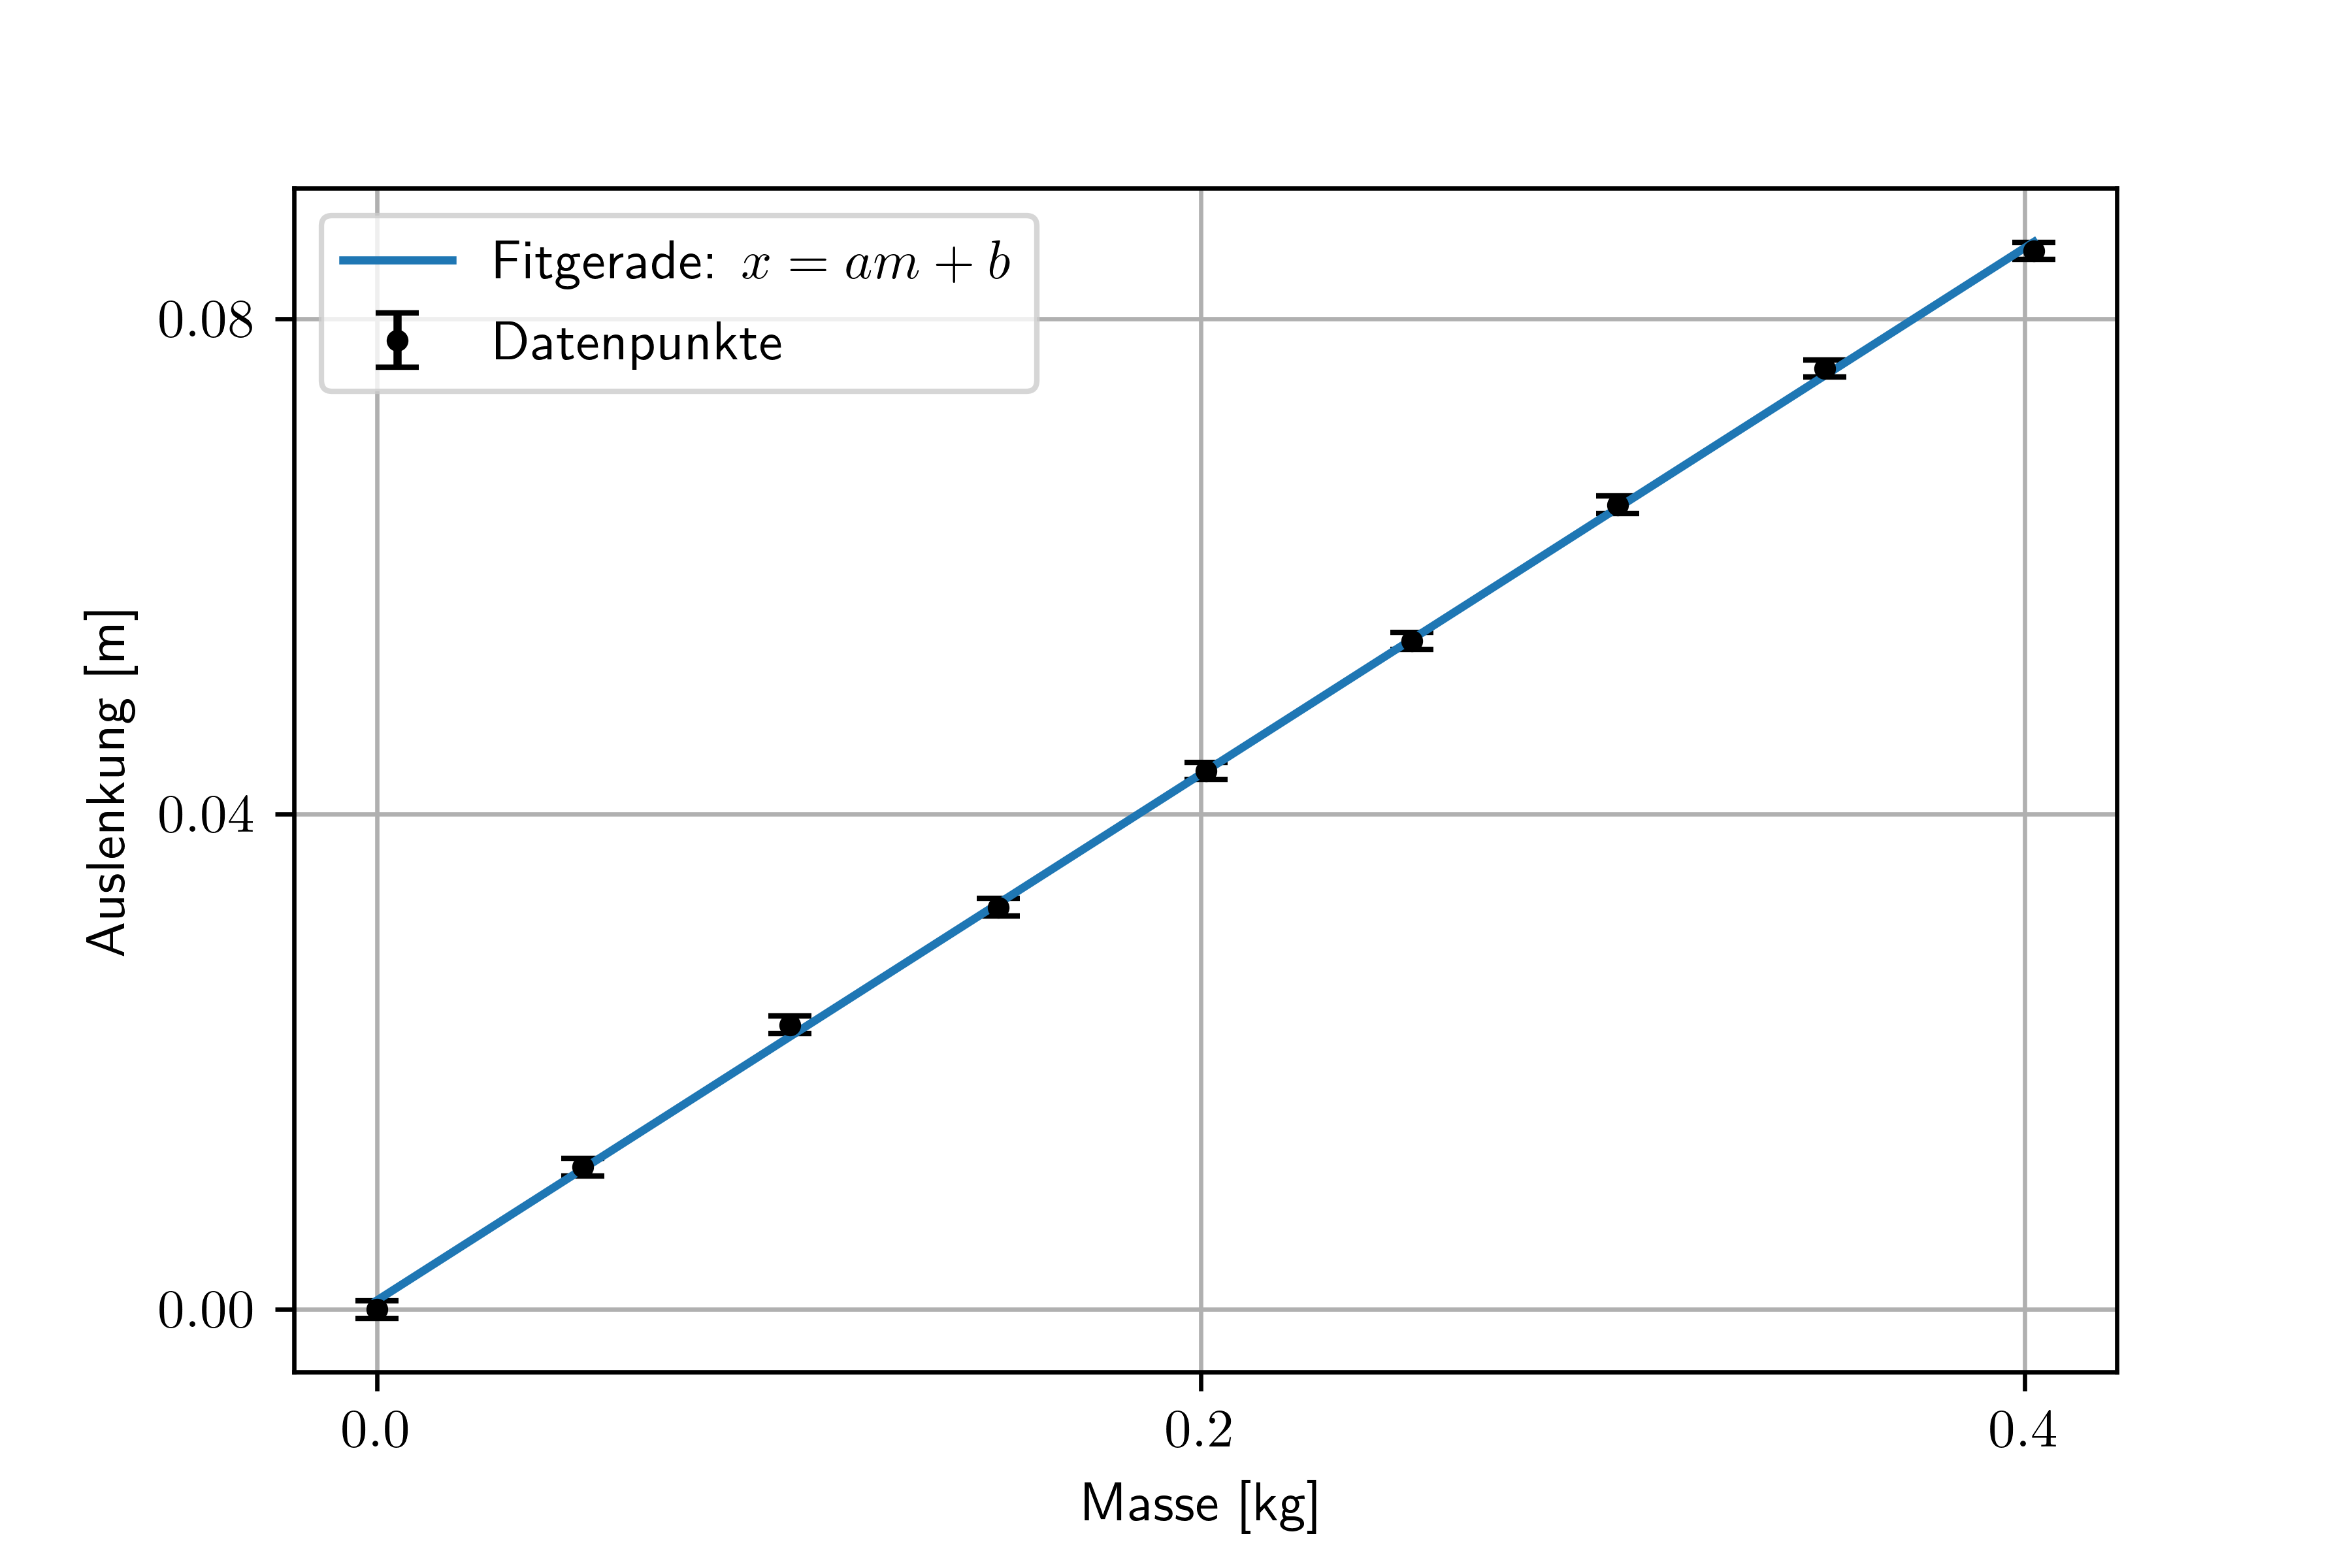
\includegraphics[width=350pt]{fotos/gpr1/B_Reg_A1_M1.png}			 
		\caption{Regeression, $ a=(0.2126\pm 0.0015) $, $ b=(7\pm 4)10^{-4} $}							 
		\label{Abb: Reg Ben A1 M1}							 
	\end{figure}
		\begin{figure}[!ht]
		\centering								 
		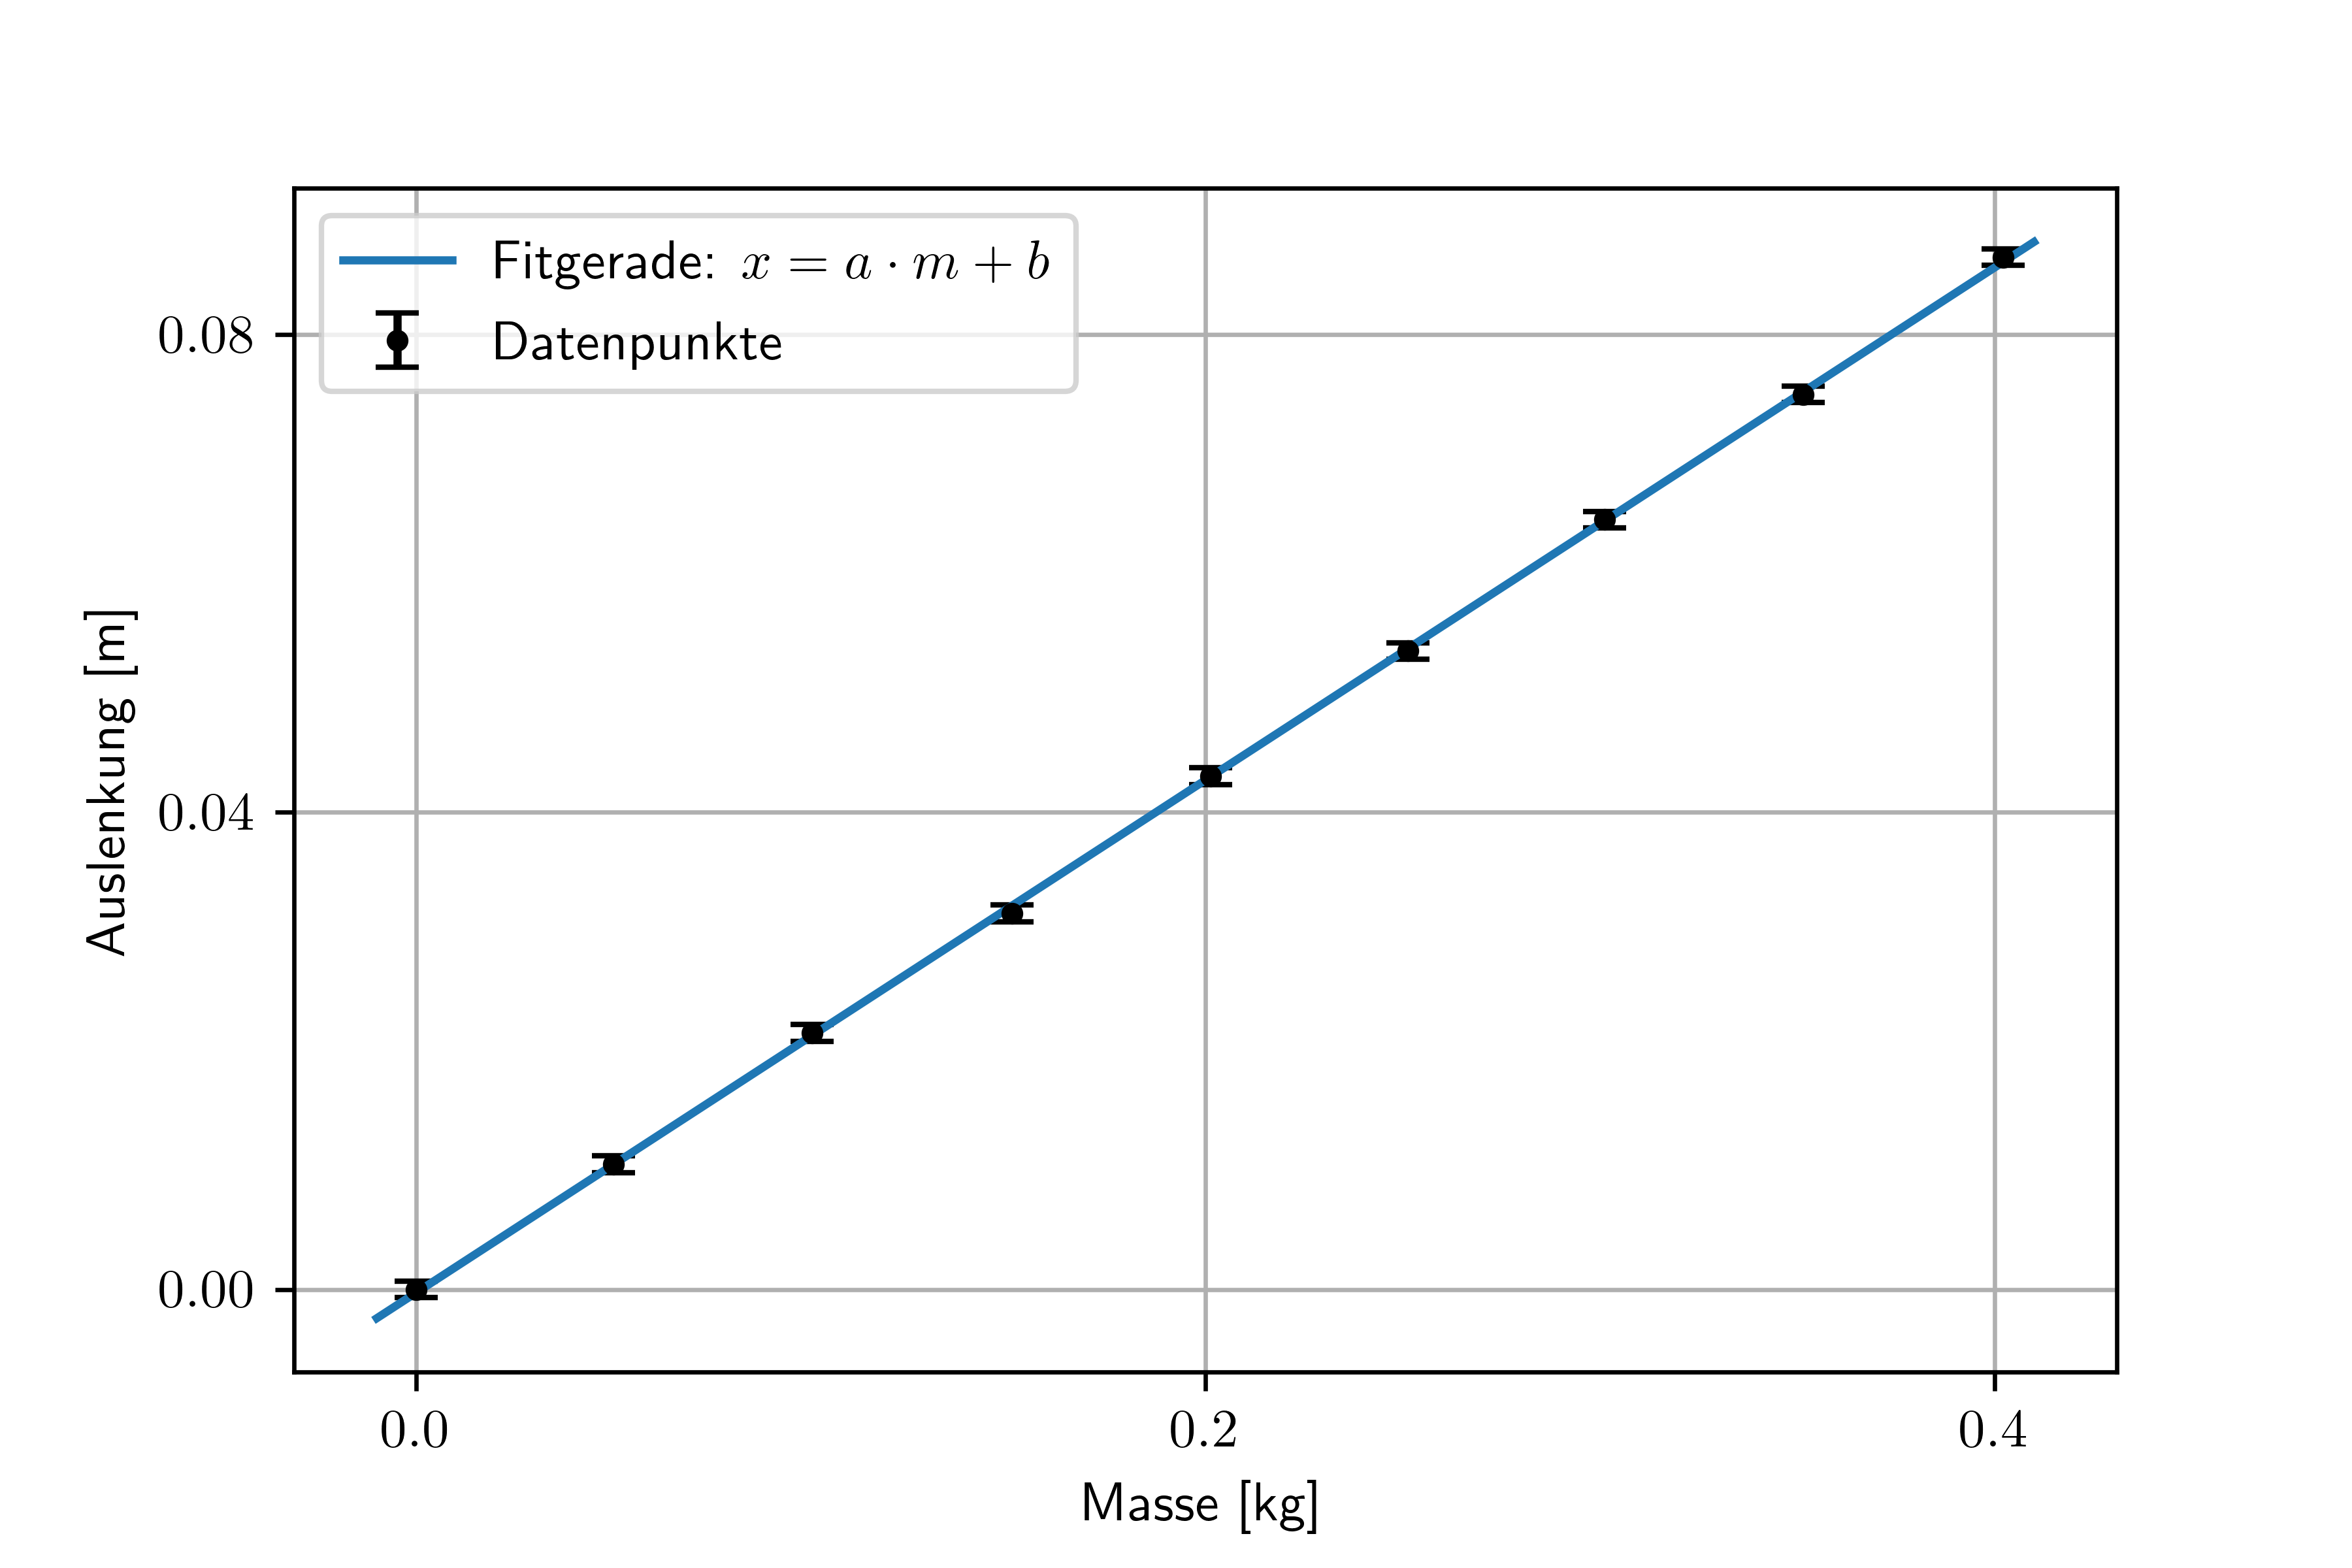
\includegraphics[width=350pt]{fotos/gpr1/B_Reg_A1_M2.png}			 
		\caption{Regeressionvon, $ a=(0.2147\pm 0.0009) $, $ b=(-2.6\pm 2.0)10^{-4} $}							 
		\label{Abb: Reg Ben A1 M2}							 
	\end{figure}
	\newpage
		\begin{figure}[!ht]
		\centering								 
		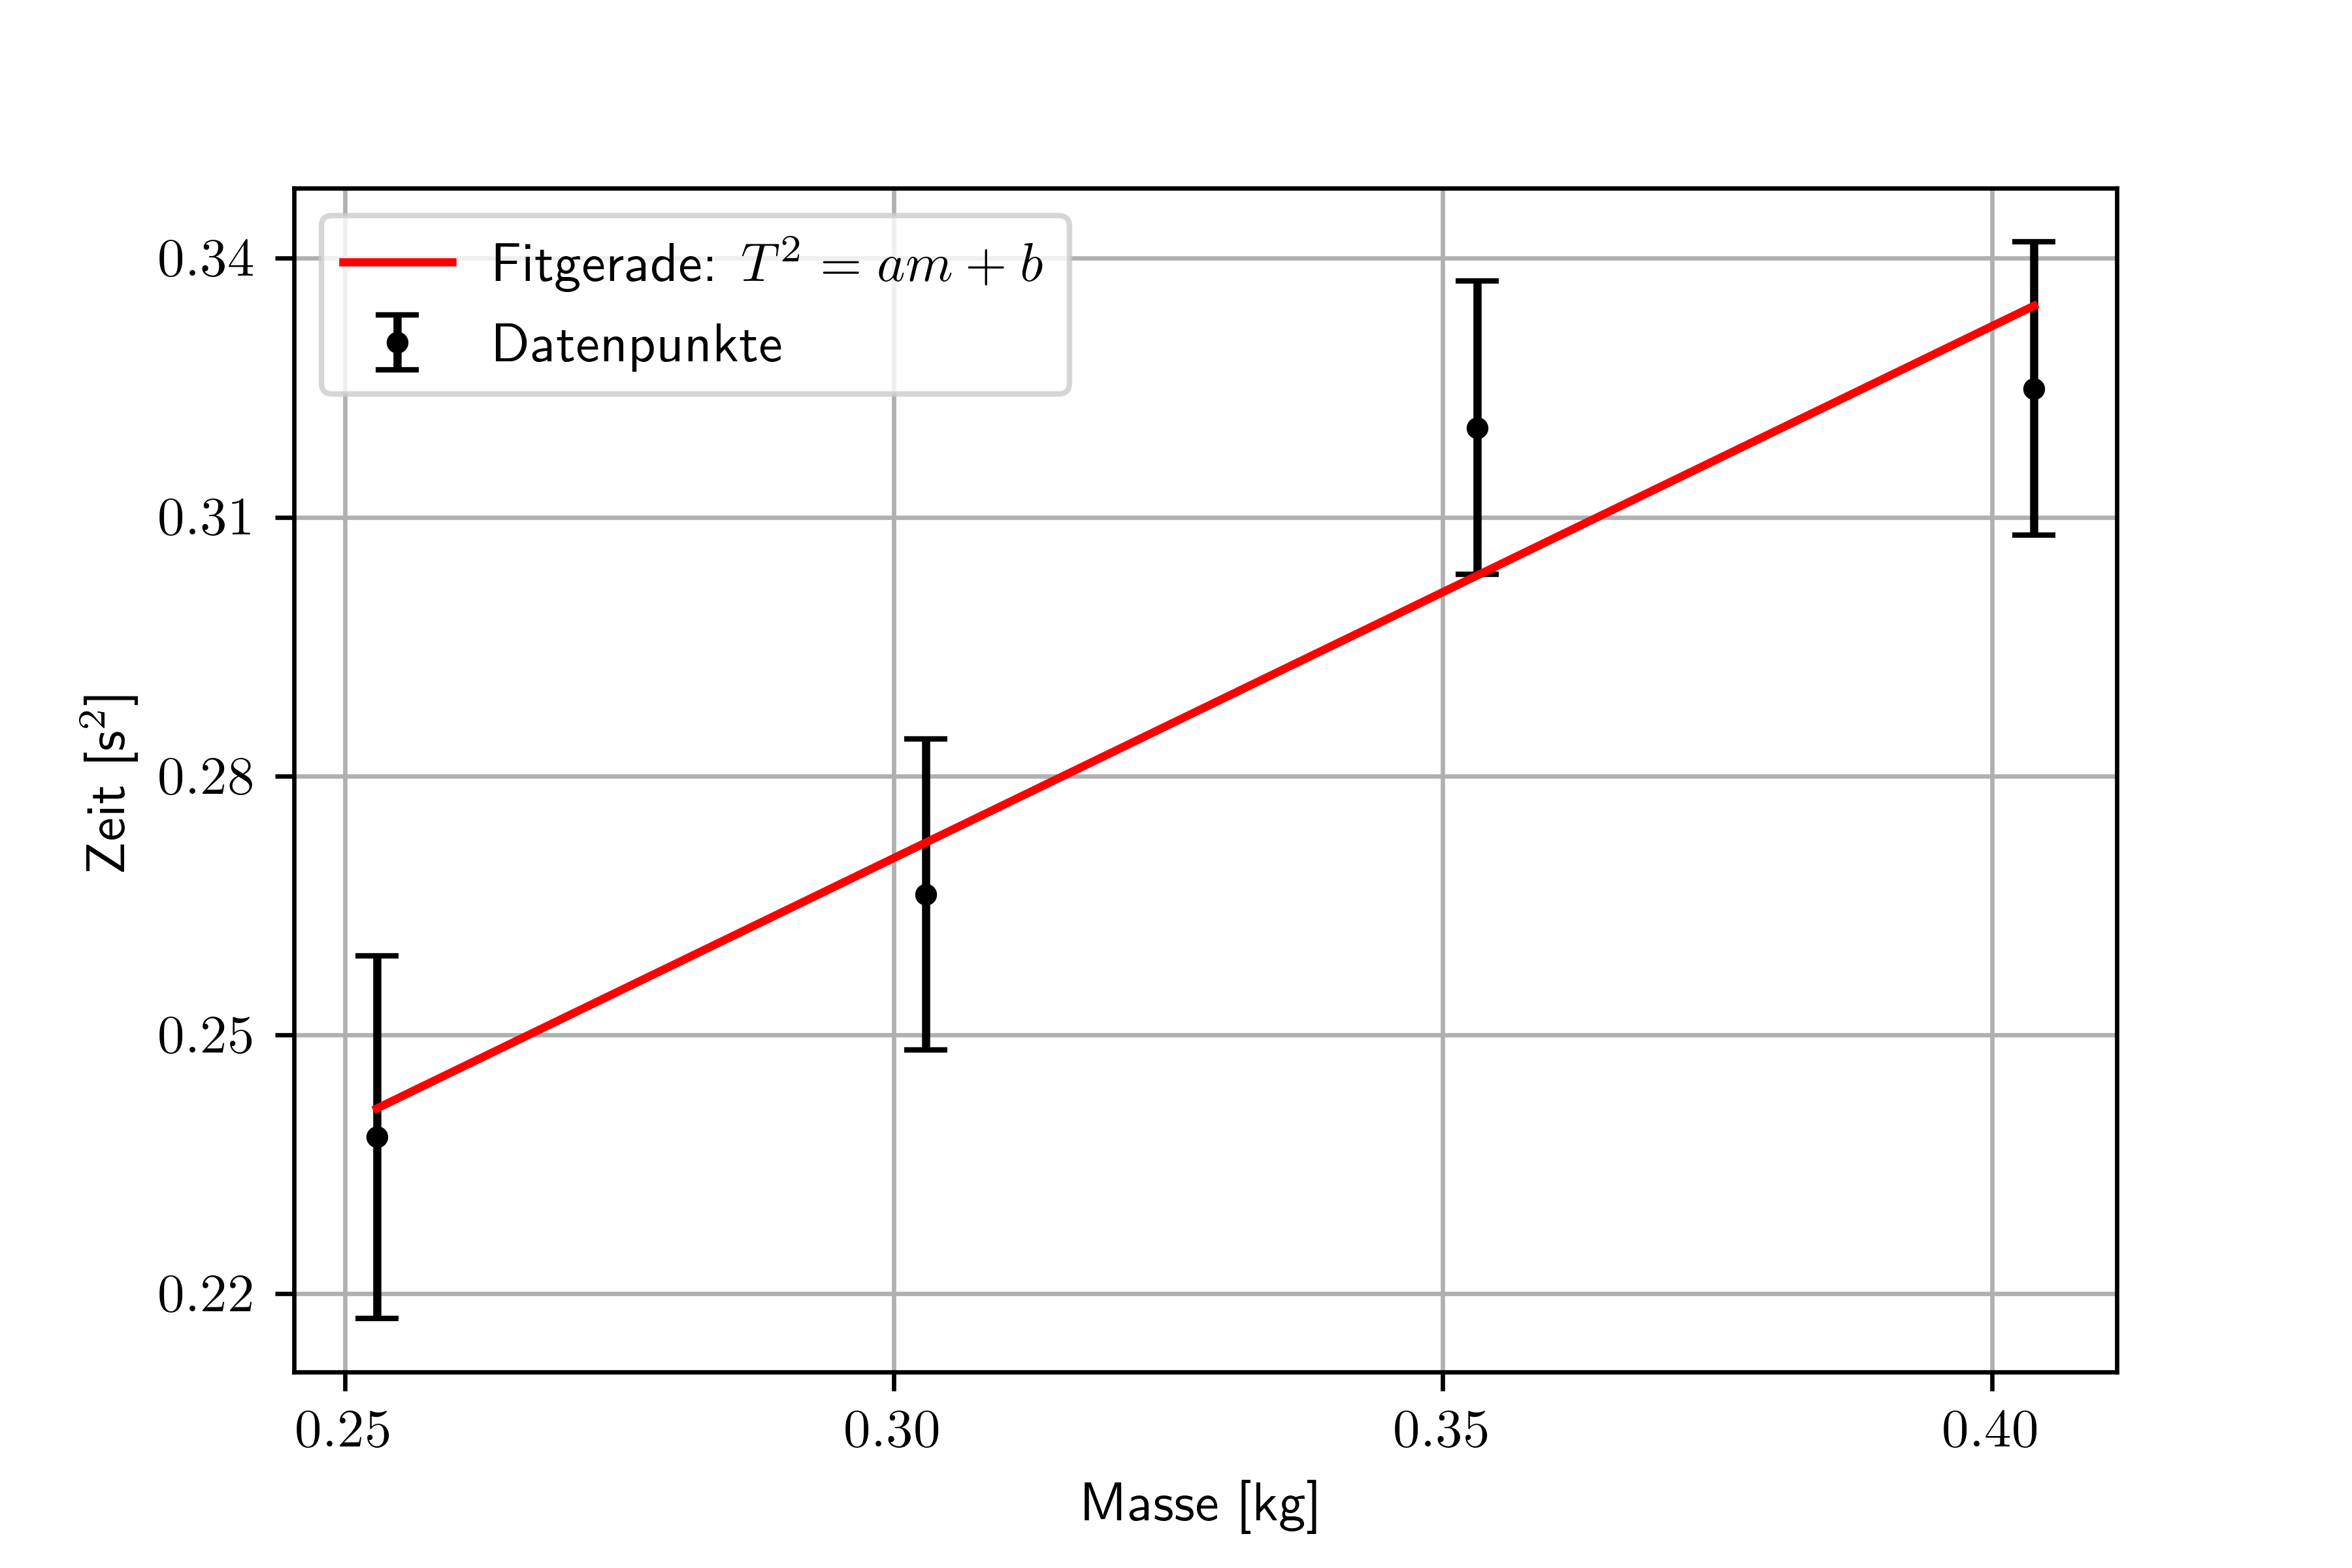
\includegraphics[width=350pt]{fotos/gpr1/B_Reg_A2.png}			 
		\caption{Regeressionvon, $ a=(0.00062\pm 0.00014) $, $ b=(9\pm 5)10^{-2} $ }							 
		\label{Abb: Reg Ben A2}							 
	\end{figure}
		\begin{figure}[!ht]
		\centering								 
		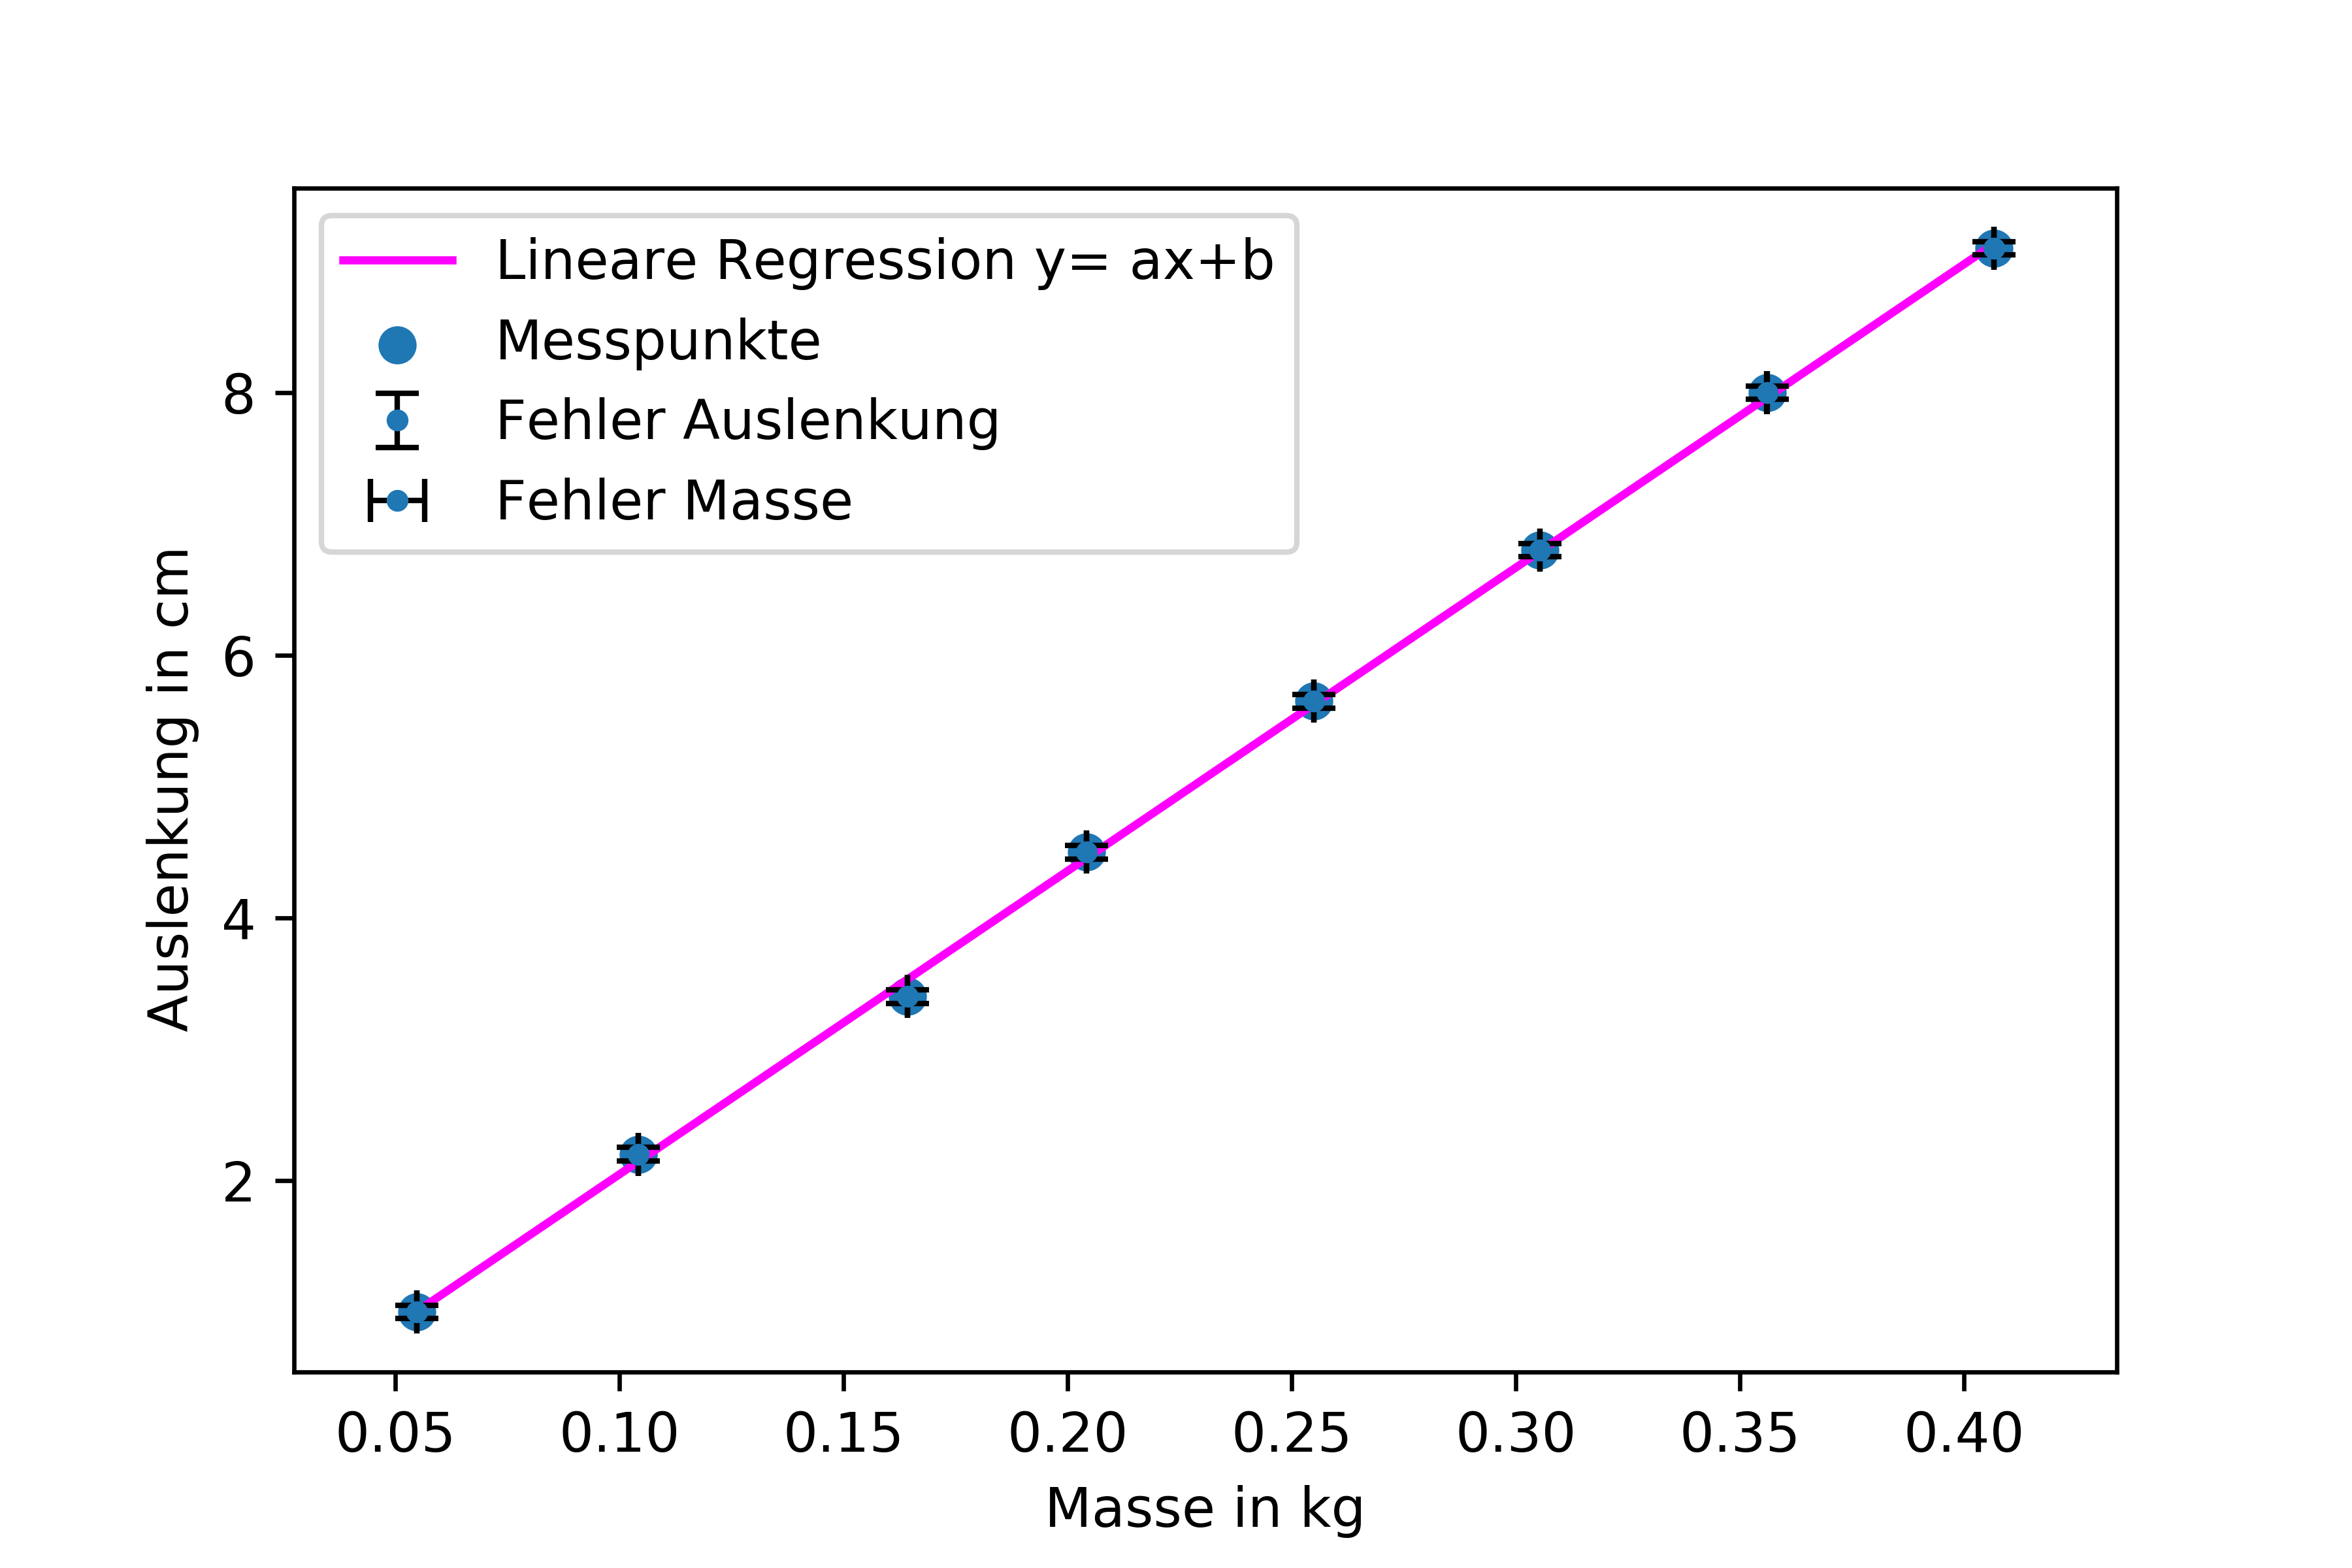
\includegraphics[width=350pt]{fotos/gpr1/S_Reg_A1.png}			 
		\caption{Regeressionvon, $ a=(23.11\pm 0.2)\text{ cm kg}^{-1} $, $ b= $}							 
		\label{Abb: Reg Sara A1}							 
	\end{figure}
	\newpage
		\begin{figure}[!ht]
		\centering								 
		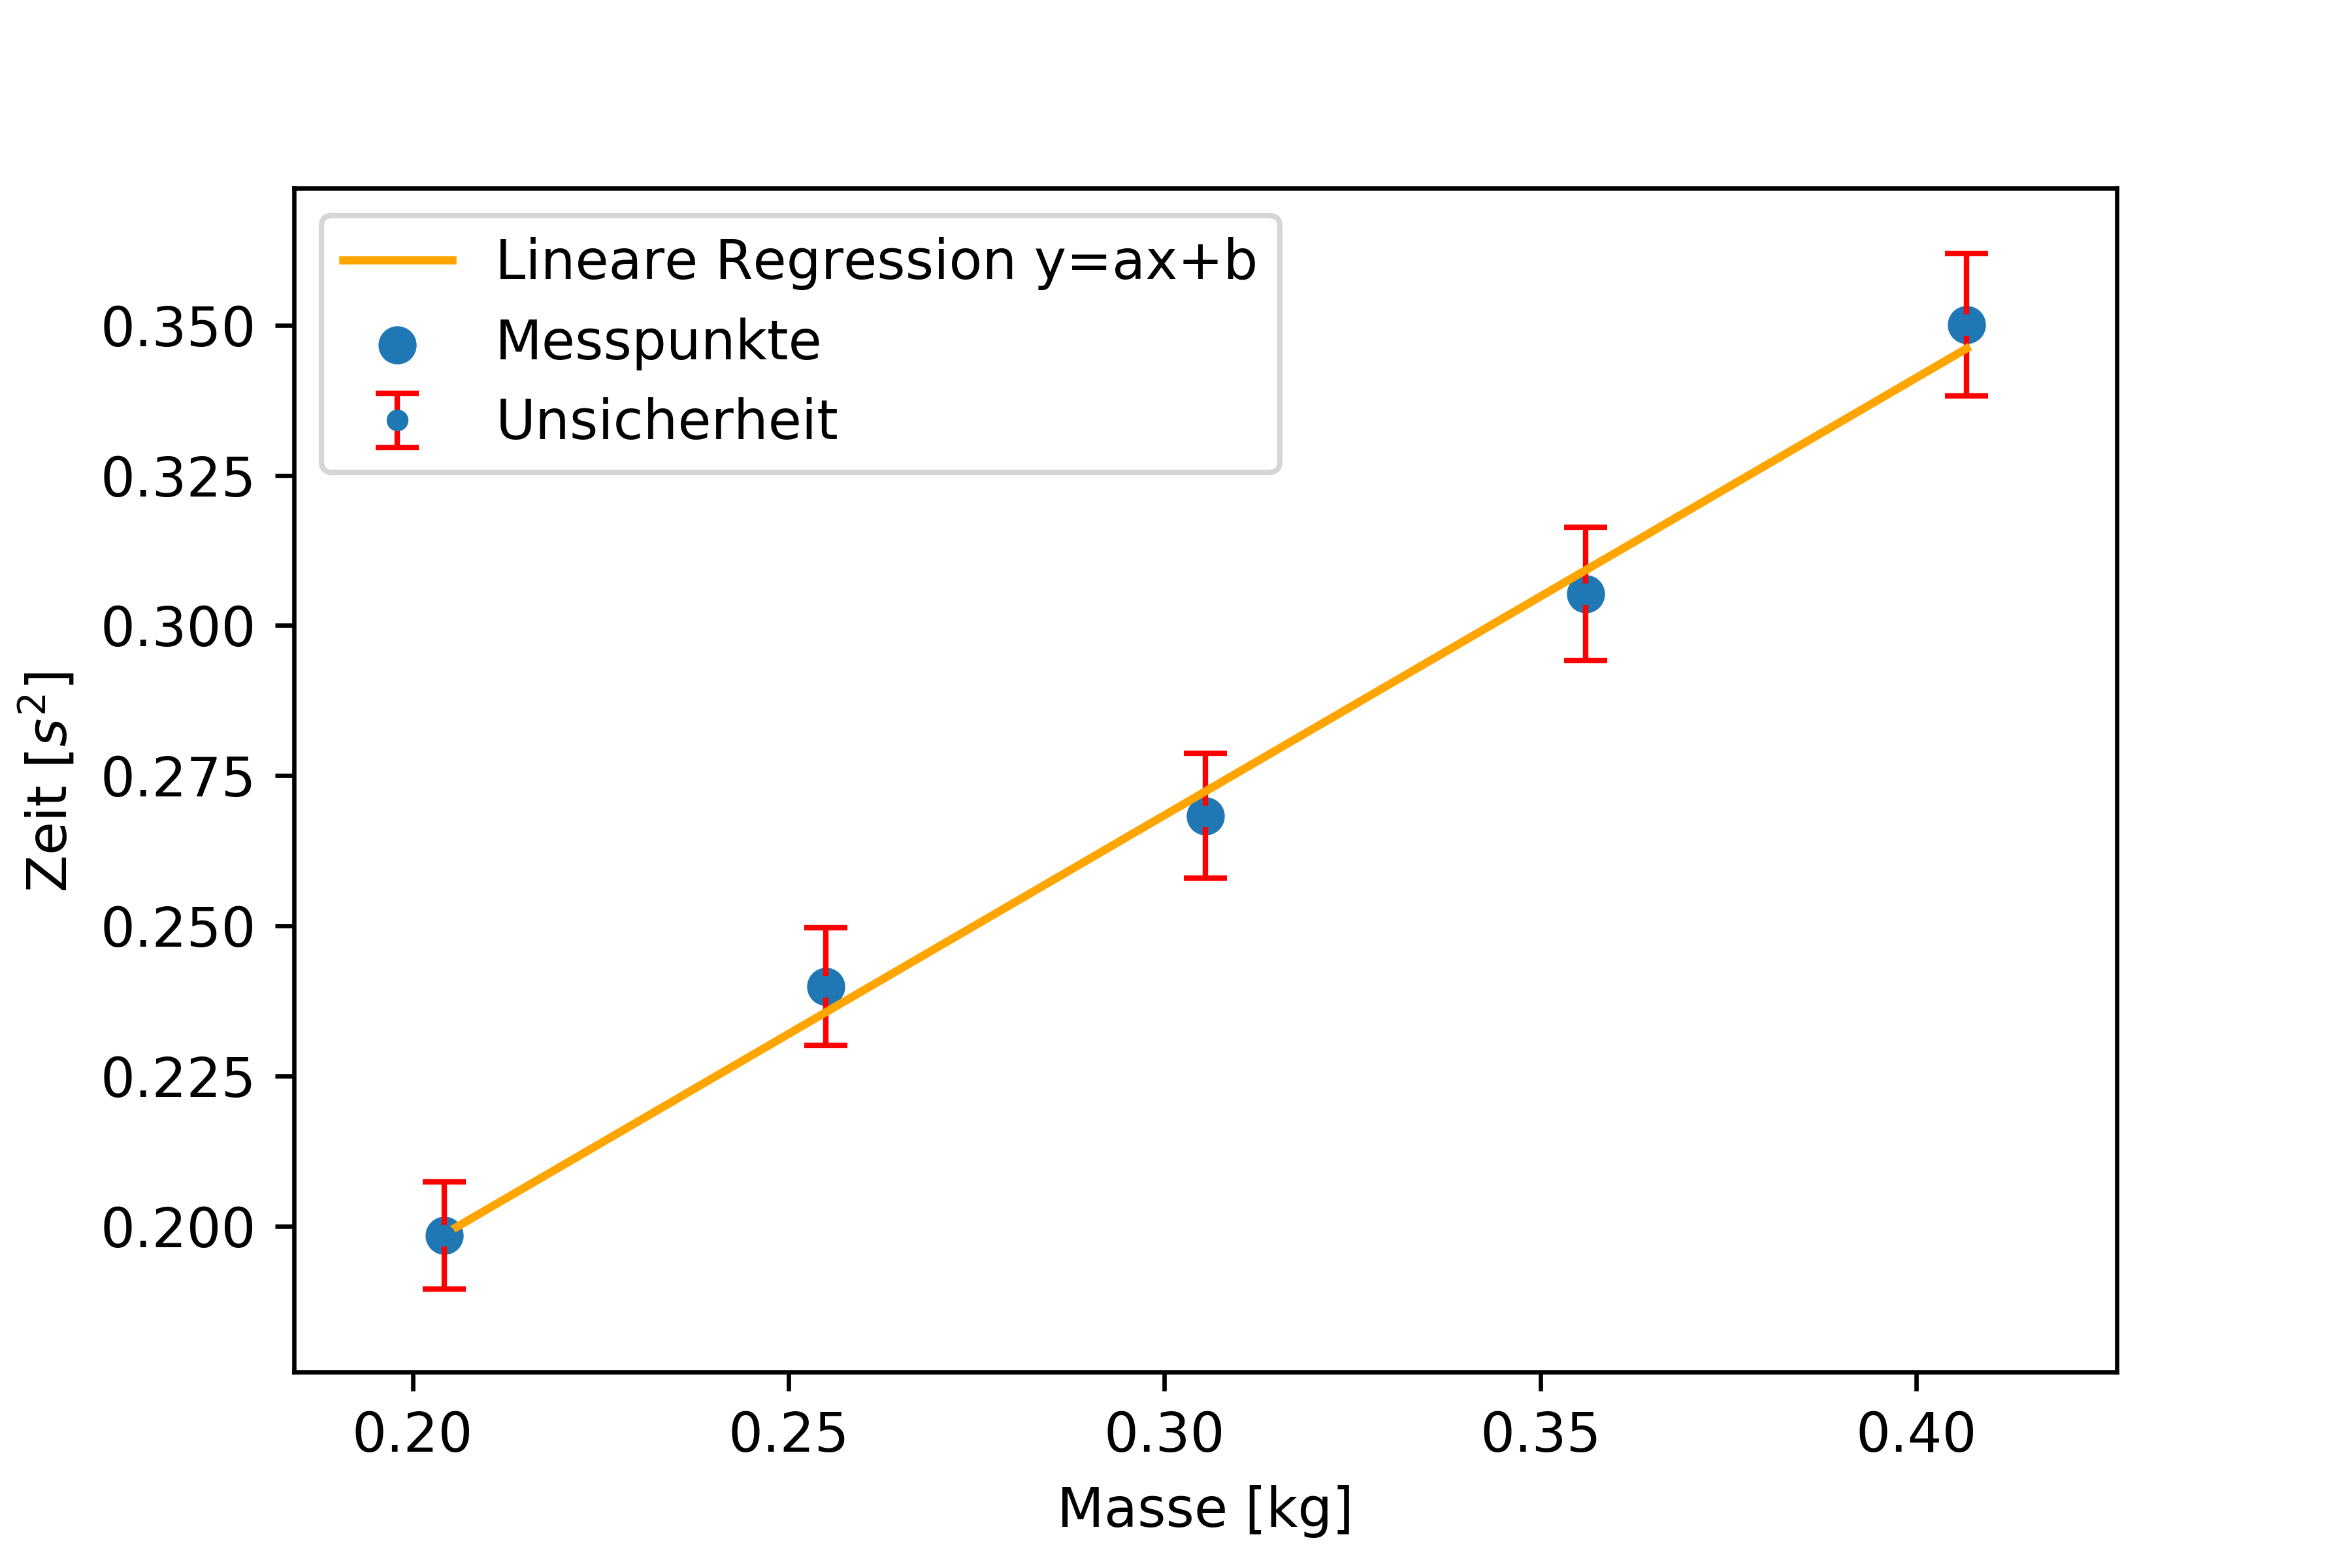
\includegraphics[width=350pt]{fotos/gpr1/S_Reg_A2.png}			 
		\caption{Regeression, S. }							 
		\label{Abb: Reg Sara A2}							 
	\end{figure}
\subsection{Chi-Quadrat Grafiken}
\begin{figure}[!ht]
	\centering								 
	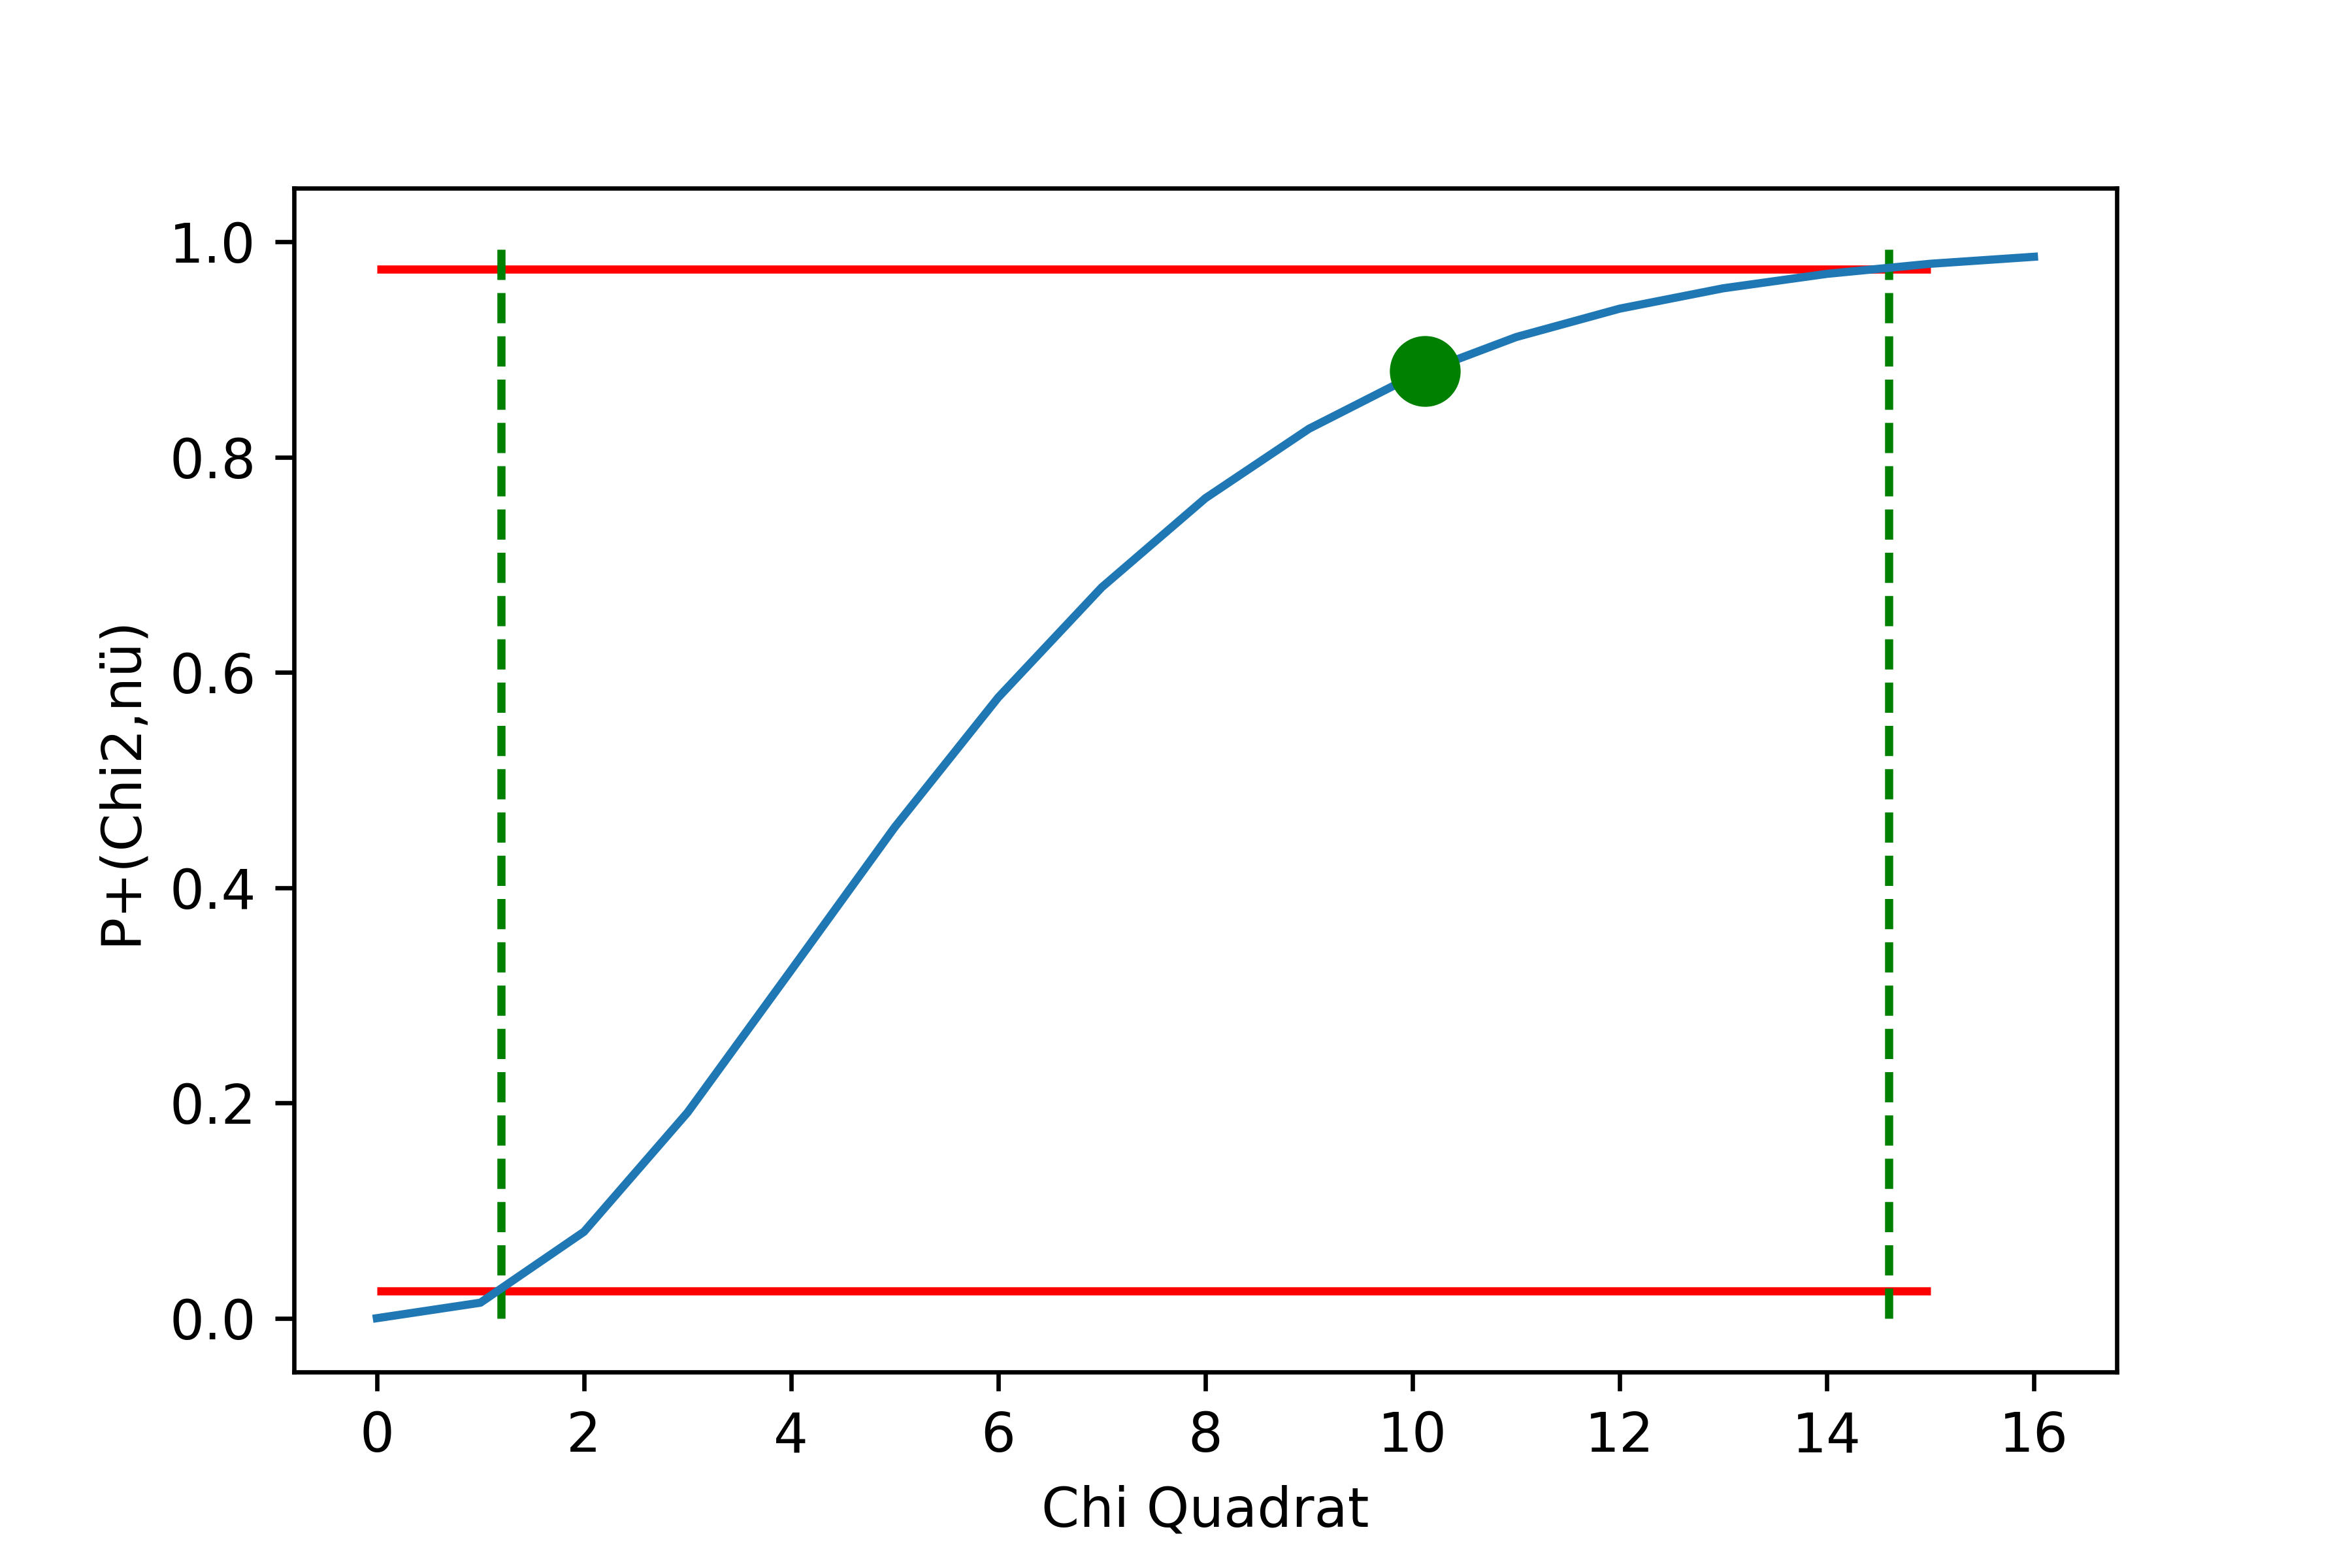
\includegraphics[width=350pt]{fotos/gpr1/kumulierte Chi Quadrat Verteilung V1.png}			 
	\caption{kumulierte Chi Quadrat Verteilung V1}							 
	\label{kumulierte Chi Quadrat Verteilung V1}							 
\end{figure}
\newpage
\begin{figure}[!ht]
	\centering								 
	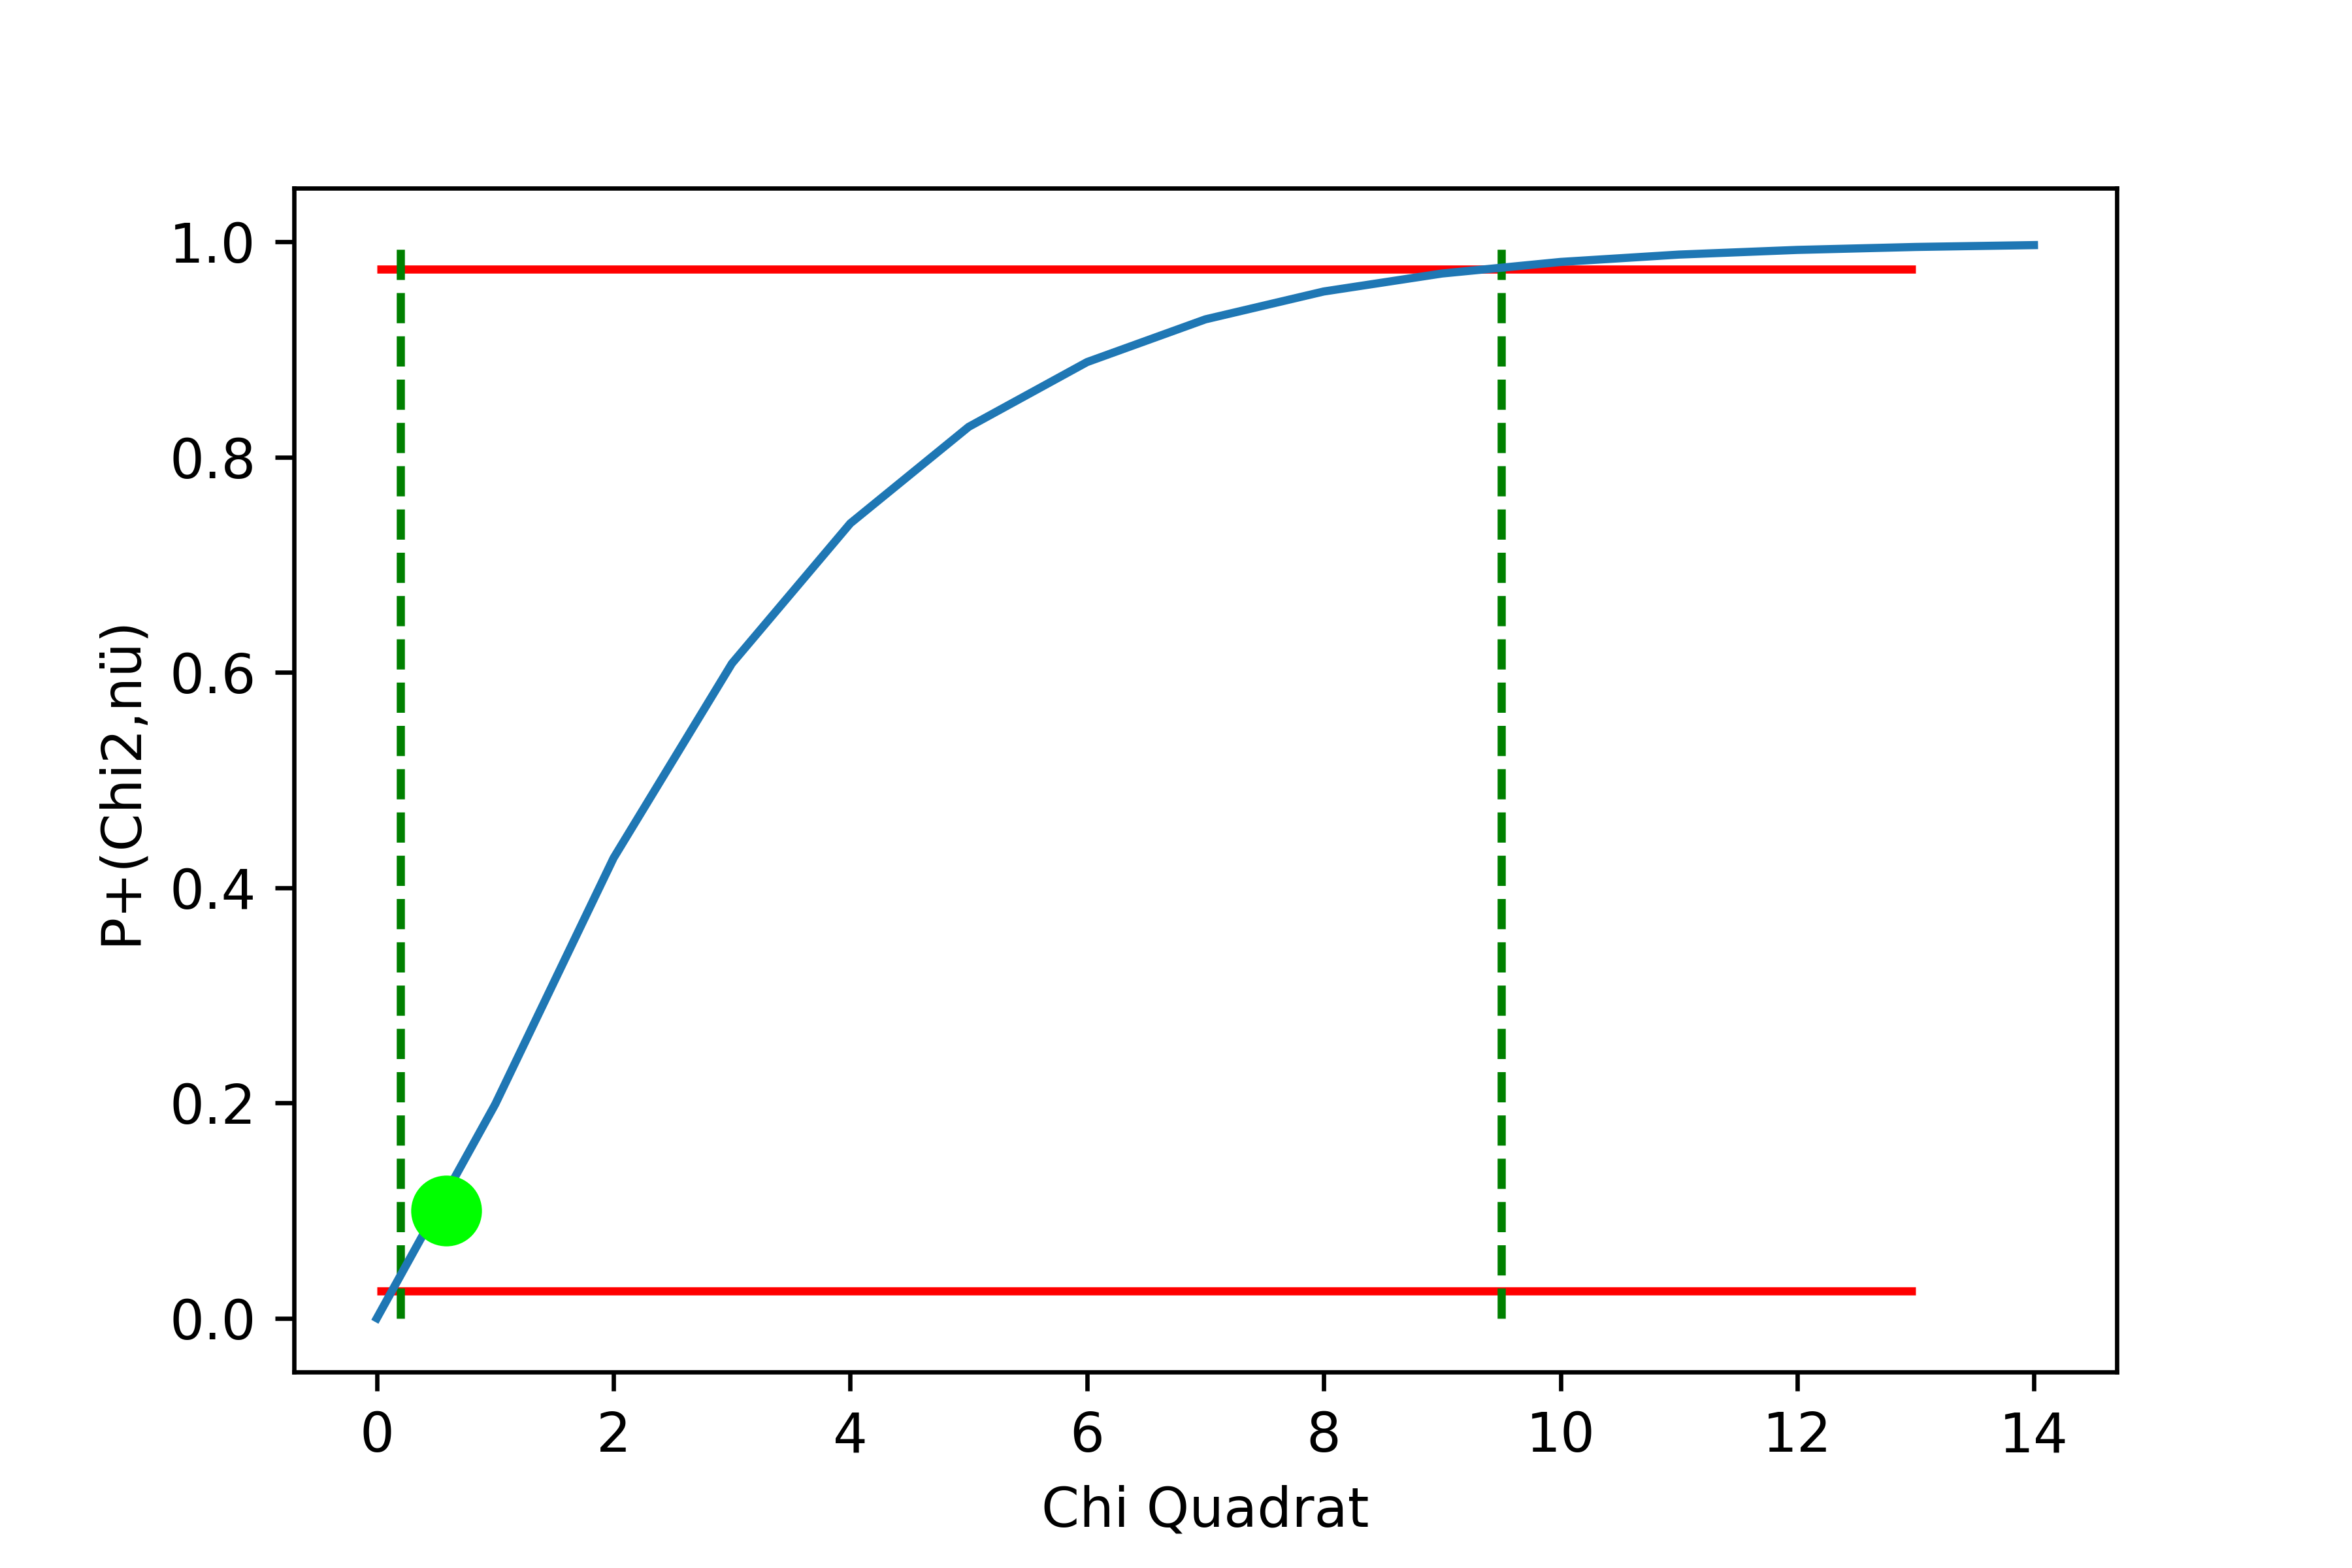
\includegraphics[width=350pt]{fotos/gpr1/kumulierte Chi Quadrat Verteilung V2.png}			 
	\caption{kumulierte Chi Quadrat Verteilung V2}							 
	\label{kumulierte Chi Quadrat Verteilung V2}							 
\end{figure}

\begin{figure}[!ht]
	\centering								 
	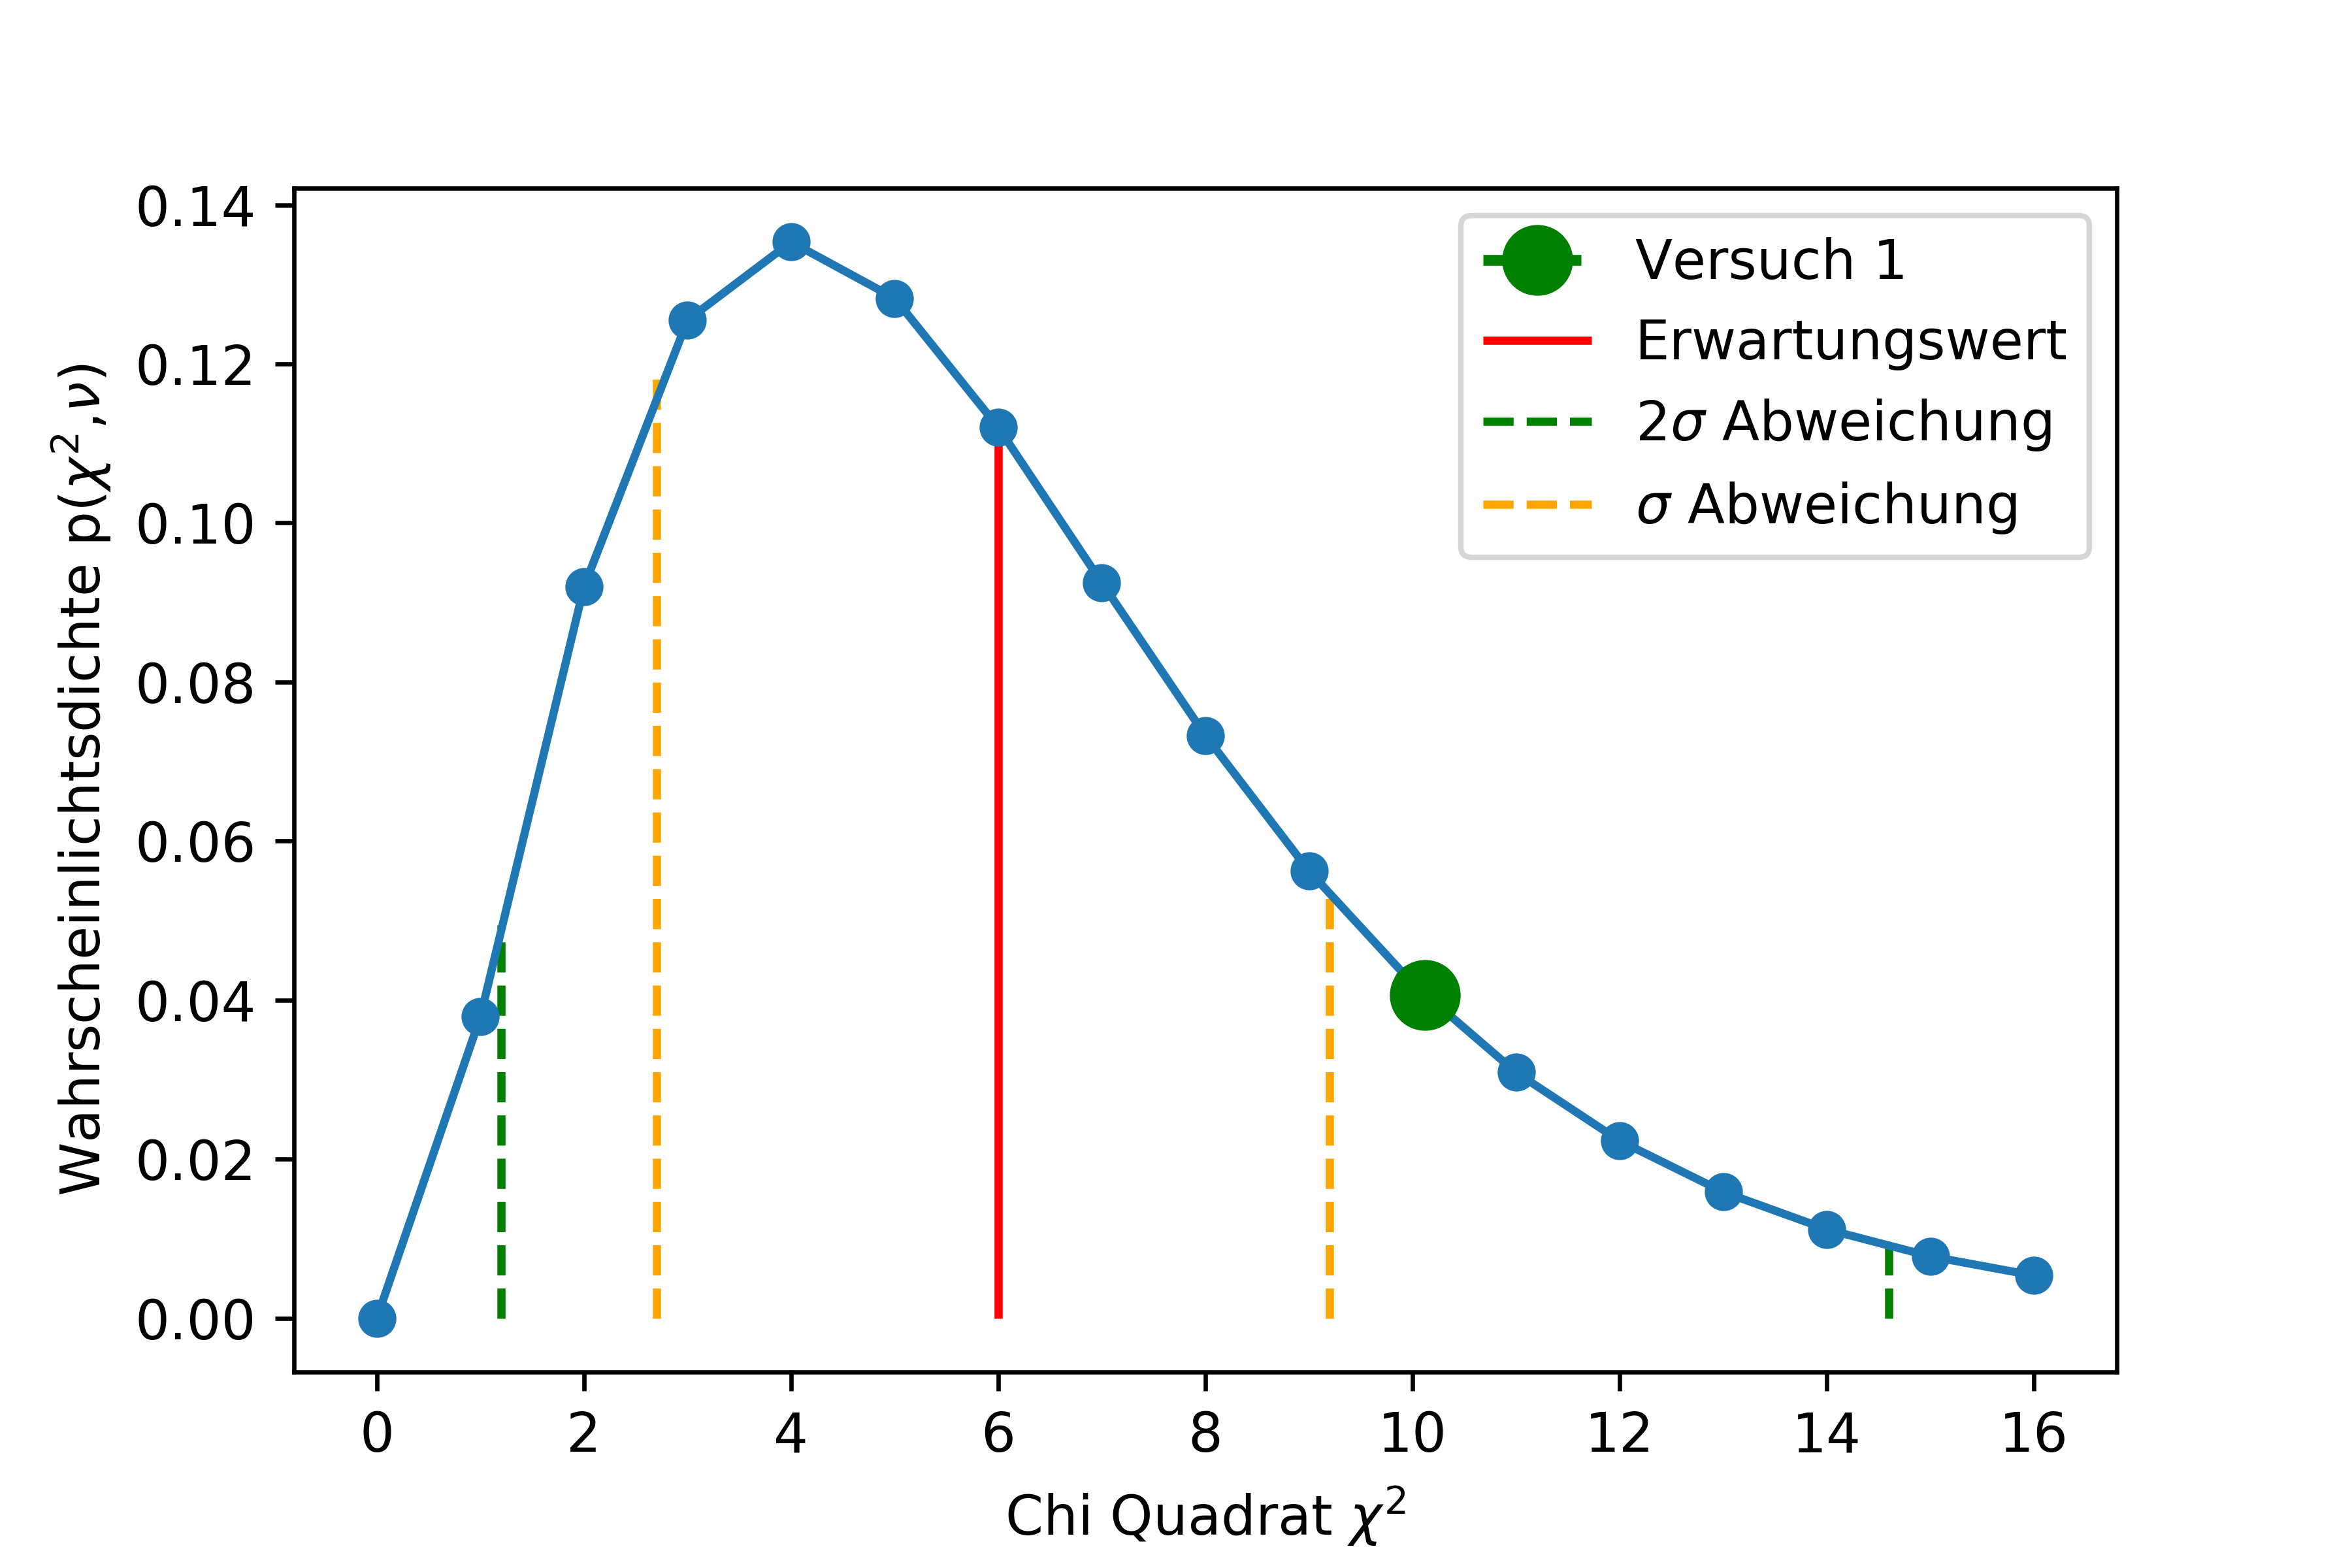
\includegraphics[width=350pt]{fotos/gpr1/Chi-Quadrat Wahrscheinlichkeitsdichte V1.png}			 
	\caption{Chi-Quadrat Wahrscheinlichkeitsdichte V1}							 
	\label{Chi-Quadrat Wahrscheinlichkeitsdichte V1}							 
\end{figure}
\newpage
\begin{figure}[!ht]
	\centering								 
	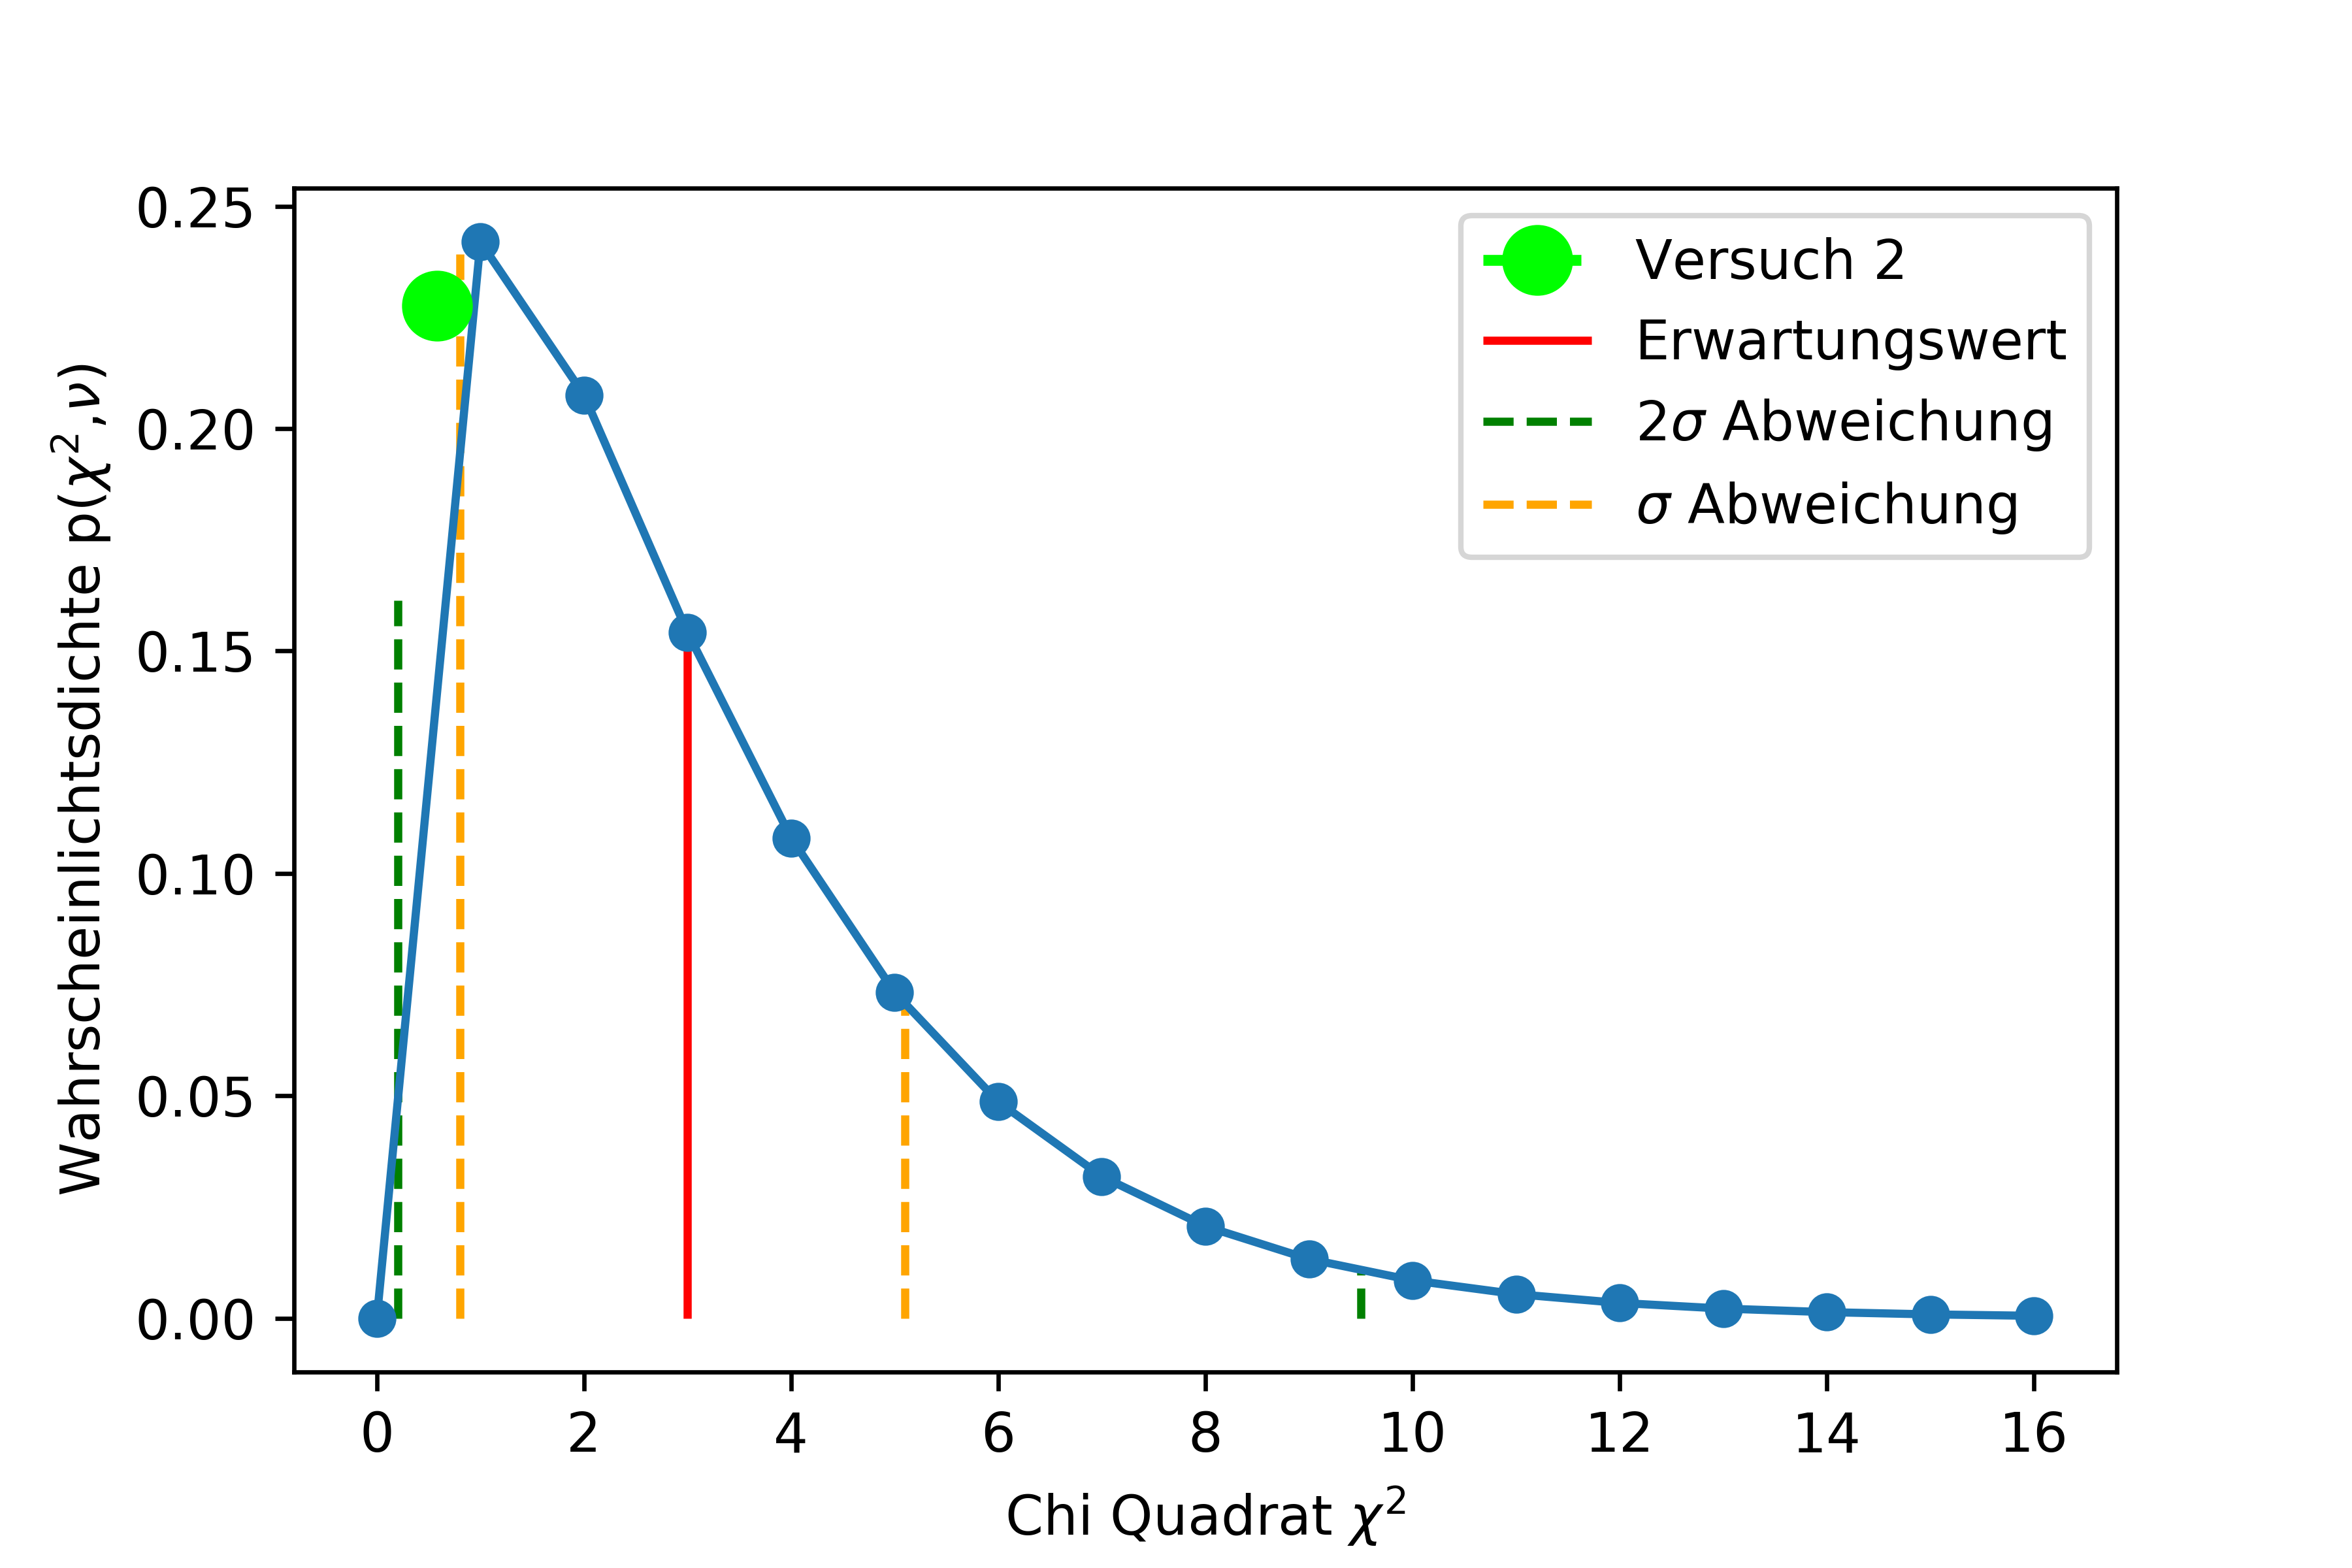
\includegraphics[width=350pt]{fotos/gpr1/Chi-Quadrat Wahrscheinlichkeitsdichte V2.png}			 
	\caption{Chi-Quadrat Wahrscheinlichkeitsdichte V2}							 
	\label{Chi-Quadrat Wahrscheinlichkeitsdichte V2}							 
\end{figure}
\begin{figure}[!ht]
	\centering								 
	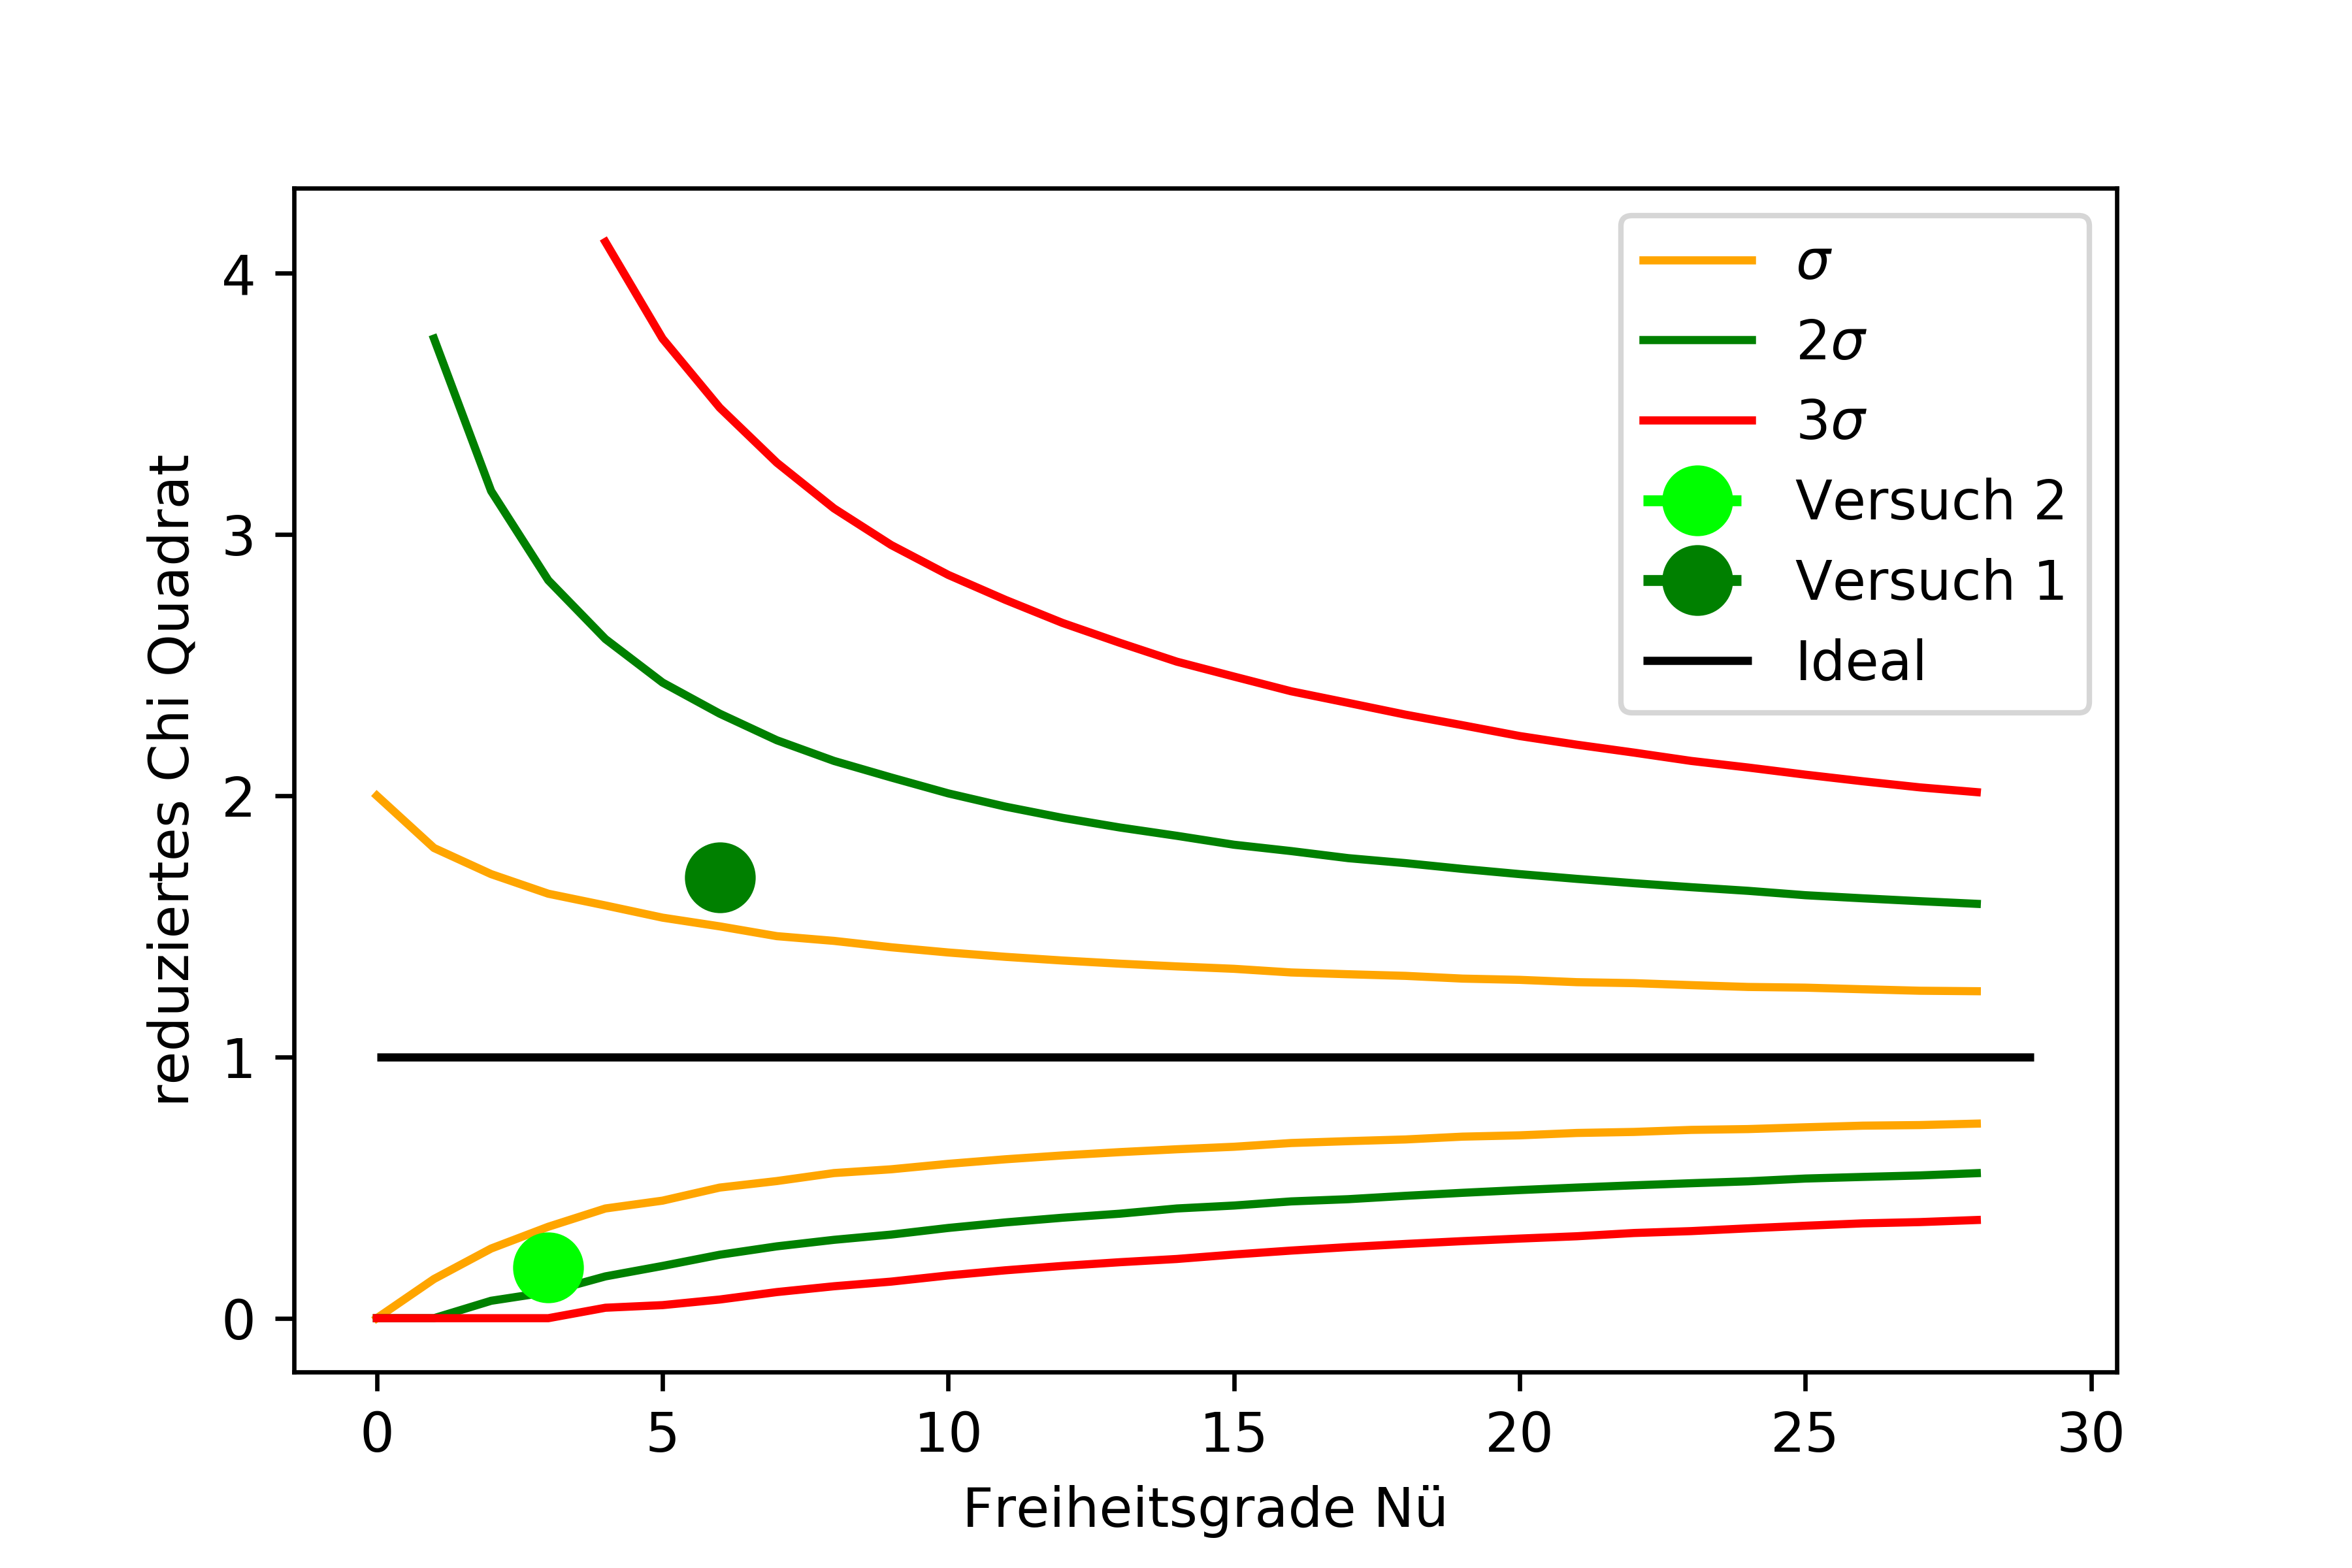
\includegraphics[width=350pt]{fotos/gpr1/Konfidenzintervall vs Freiheitsgrade im reduzierten Chi Quadrat.png}			 
	\caption{Konfidenzintervall vs Freiheitsgrade im reduzierten Chi Quadrat}							 
	\label{Konfidenzintervall vs Freiheitsgrade im reduzierten Chi Quadrat}							 
\end{figure}


	\newpage
	\printbibliography[title={Quellenverzeichnis}]
	
	
\end{document}